\documentclass[aps,12pt,superscriptaddress,nofootinbib,floatfix,showpacs]{revtex4}
%\documentclass[aps,prl,twocolumn,nofootinbib,superscriptaddress]{revtex4}
%\documentclass[aps,prl,twocolumn,nofootinbib]{revtex4}
%\documentclass[showpacs,preprintnumbers,amsmath,amssymb,12pt]{revtex4} 
\usepackage{graphicx}
\usepackage{amssymb} 
\usepackage{amsmath} 
\usepackage{color} 
\usepackage{axodraw}
\renewcommand{\bottomfraction}{0.99} 
\renewcommand{\topfraction}{0.99} 
\renewcommand{\textfraction}{0.01}


%%%%%%%%%%% To get line numbers: %%%%%%%%%%%%%%%
%\documentclass[12pt,twoside,letterpaper,doublespace]{article}%
%\topmargin -0.25cm
%\textwidth 15.5cm
%\textheight 22cm
%\oddsidemargin 0.5cm
%\evensidemargin 0.5cm%

%%%%%%%%%%%%%%%%%%%%%%%%%%%%%%%%%%%%%%%

\usepackage{dcolumn}% Align table columns on decimal point





\input phys_def.tex

\begin{document}

\title
{LHC discovery potential 
of the lightest NMSSM Higgs in $h \to a_a \to \mu \mu \mu \mu$
channel}

\author{Alexander Belyaev}
\affiliation{
School of Physics \& Astronomy, University of Southampton,\\
Highfield, Southampton SO17 1BJ, UK}
\affiliation{
Particle Physics Department, Rutherford Appleton Laboratory, \\Chilton,
Didcot, Oxon OX11 0QX, UK
}
\author{Jim Pivarski}
\affiliation{Physics Department, Texas A\&M University}
\author{Alexei Safonov}
\affiliation{Physics Department, Texas A\&M University}
\author{Sergey Senkin}
\affiliation{Physics Department, Texas A\&M University}

%\affiliation{URL http://www-cdf.fnal.gov}

\date{\today}
%\maketitle


\begin{abstract}
We explore the potential of Large Hadron Collider to observe  $h_1\to
a_1a_1\to 4\mu$ signal from the lightest lightest scalar Higgs boson
($h_1$) decaying into two  lightest pseudoscalar Higgs bosons($a_1$) 
followed by their decays into 4 muons within the Next-to-Minimal
Supersymmetric Standard Model (NMSSM).
The signature under study allows to cover the  NMSSM parameter space
with  $M_{a_1}$ below 3.5 GeV and large $Br(h_1\to a_1 a_1)$ 
which has not been studied previously. In case of  such a scenario,
the suggested strategy of the observation of 
$4\mu$ signal with the respective background suppression
would provide a unique way to discover
the lightest scalar NMSSM Higgs boson.
\end{abstract}

% activate the following line for publication
\pacs{13.38.Dg 13.38.Qk}

\maketitle
\newpage
\tableofcontents
\newpage

%
\section{Introduction}

The next-to-minimal supersymmetric standard model (NMSSM)
\cite{Nilles:1982dy,Frere:1983ag,Ellis:1988er,%
Drees:1988fc,Ellwanger:1993hn,Ellwanger:1993xa,%
Elliott:1993bs,Pandita:1993tg,Ellwanger:1995ru,%
King:1995vk,Franke:1995tc,Ellwanger:1996gw,Miller:2003ay}
is extended by one singlet superfield in addition to the particle content
of the Minimal Supersymmetric Standard Model (MSSM)
and due to this design 
has several new attractive features as compared to MSSM.
First  of all, NMSSM elegantly solves so called $\mu$-problem~\cite{mu-problem}:
the scale of the $\mu$-parameter is automatically generated 
at the electroweak or SUSY  scale when the singlet Higgs acquires 
a vacuum expectation value.
On the other hand NMSSM can solve fine-tuning and little hierarchy problems
of MSSM~\cite{Dermisek:2005ar}.
The upper mass limit on the lightest  CP-even
Higgs boson in NMSSM is larger than in MSSM and since more
parameter space survives LEP II bounds from the Higgs search,  NMSSM
is less fine-tuned.
On the other hand  there is additional mechanism for the reduction of
fine-tuning since 
LEP II bounds from the Higgs search can be partly avoided if the
branching of  $h_1\to a_1 a_1$ decay is significant ($h_1$ and
$a_1$ stands for the lightest   CP-even  and CP-odd Higgs bosons respectively).
This decay channel of $h_1$ diminishes the branching ratios for
conventional modes used in direct Higgs  searches and largely softens
direct Higgs boson mass limits from LEP. 

One should stress that due to the extended scalar sector (in comparison to MSSM)
NMSSM offers richer Higgs collider phenomenology
\cite{nmssm-ph1,nmssm-ph2,%
nmssm-ph2b,nmssm-ph3,nmssm-ph4,%
nmssm-ph5,nmssm-ph6,nmssm-ph6a,nmssm-ph7}
as well as richer  cosmological Dark Matter implications 
related to the presence of the fifth  neutralino (``singlino"),
relic density for  which can be achieved to be correct one~\cite{nmssm-dm}.

The collider phenomenology of the Higgs sector of the NMSSM
is very interesting in several aspects, therefore a short historical 
introduction is in  order.
In \cite{nmssm-ph2} the first attempt to establish `no-lose' theorem for NMSSM
has been done. This theorem states that LHC has a potential to discover at least one
NMSSM Higgs boson in the conventional mode given that Higgs-to-Higgs decay modes 
are not important. However the point is that  Higgs-to-Higgs decay modes
can be important as has been shown and studied later on
in analysis devoted to re-establishing   of `no-lose' 
theorem~\cite{nmssm-ph2b,nmssm-ph3,nmssm-ph4,nmssm-ph5,nmssm-ph6,nmssm-ph6a,nmssm-ph7}
for the case when  $h_1\to a_1 a_1$ decay is significant
and $a_1$ is light. So far, the case of the lightest $a_1$  was explored 
for $m_{a_1}$ below $2b$-quark threshold but above $2\tau$ one,
$2m_\tau <m_{a_1}<2m_b$, establishing the scope of
the $4\tau$ channel in Higgs-strahlung and Vector Boson Fusion
for the NMSSM No-Lose Theorem at the LHC~\cite{nmssm-ph7}.
Theses analysis  require a substantial integrated luminosity (10-100 fb$^{-1}$)
and quite challenging analysis in the technical sense.


In this paper we explore the  mass region of  $a_1$ 
with the mass below $2\mu$ threshold: $m_{a_1}<2m_\mu$.
In this case, which has not been studied previously, we 
explore $h_1 \to a_1a_1 \to \mu \mu \mu \mu$ signature.
Unlike searches for $4\tau$ signature,
the measurement of invariant mass of muon pair provides a 
direct estimate of $m_{a_1}$ which defines a clear set of the kinematical
cuts for the background suppression. 
Further, this
channel is essentially free of backgrounds and therefore allows to use
direct gluon fusion production combined with  $b\bar{b}$ fusion production
instead of subdominant  vector boson fusion or associate 
Higgs production processes used in case of $4\tau$ signature to to suppress large QCD
backgrounds.

We demonstrate that the analysis in
the four muon mode has excellent sensitivity for Lightest CP-even NMSSM Higgs boson
and can be performed with just  a handful of first CMS data and requires 
very little in terms of detector performance  except reasonably robust tracking 
for muons and well functioning muon system. To make 
this a realistic analysis, we use parameters of the CMS experiment in designing
selections and estimating background contributions.

The rest of the paper is organized as follows.
In Section II we study the NMSSM parameters space 
for which $m_{a_1}<2m_\mu$ case of our study is realized.
In Section III we perform signal versus background analysis
and present our final  results in Section IV.
In Section V we draw our conclusions.


%%%%%%%%%%%%%%%%%%%%%%%%%%%%%%%%%%%%%%%%%%%%%%%%%%%%%%%%%%%%%%%%%%%%%%
%%%%%%%%%%%%%%%%%%%%%%%%%%%%%%%%%%%%%%%%%%%%%%%%%%%%%%%%%%%%%%%%%%%%%%
%%%%%%%%%%%%%%%%%%%%%%%%%%%%%%%%%%%%%%%%%%%%%%%%%%%%%%%%%%%%%%%%%%%%%%
%%%%%%%%%%%%%%%%%%%%%%%%%%%%%%%%%%%%%%%%%%%%%%%%%%%%%%%%%%%%%%%%%%%%%%

\section{NMSSM Parameter Space and Signal production rates}

\subsection{The model and the parameter space for  the light $a_1$ scenario}
In our study we consider the simplest version of NMSSM
\cite{Nilles:1982dy,Frere:1983ag,Ellis:1988er,%
Drees:1988fc,Ellwanger:1993hn,Ellwanger:1993xa,%
Elliott:1993bs,Pandita:1993tg,Ellwanger:1995ru,%
King:1995vk,Franke:1995tc,Ellwanger:1996gw},
where $\mu\widehat{H_1}\widehat{H_2}$ term of the 
MSSM superpotential is replaced by
\begin{equation}
\lambda  \widehat{S} \widehat{H}_1 \widehat{H}_2 + \frac{\kappa}{3}  \widehat{S}^3 
\label{eq:superpot} 
\end{equation}
which makes superpotential scale invariant. In addition, we have five
soft braking terms in general,  "non-universal" case:
\begin{equation}
  m_{H_1}^2 H_1^2 + m_{H_2}^2 H_2^2  + m_{S}^2 S^2 
+ \lambda A_\lambda H_1 H_2 S +  \frac{\kappa}{3} A_\kappa S^3.
\label{eq:soft} 
\end{equation}
In the above equations the tilded capital letters denote superfield
while non-tilded ones stand for the scalar component of the respective
superfield.


Soft breaking parameters
$m_{H_1}^2$ , $m_{H_2}^2$  and $m_{S}^2$ 
from Eq.~\ref{eq:soft} can  be traded for 
$M_Z$, the ratio  of the doublet Higgs vacuum expectation values (VEVs) $\tan\beta$,
and $\mu = \lambda \langle S \rangle$
(where $\langle S \rangle$ denotes the VEV of the singlet Higgs field)
through the three minimization equations of the Higgs potential.
Therefore, 
assuming that the Higgs sector is CP conserving,
the NMSSM Higgs sector at the Electro-Weak (EW) scale is uniquely defined
by fourteen parameters:
$\tan\beta$,
the trilinear couplings in the superpotential $\lambda$ and $\kappa$, the
corresponding soft SUSY breaking parameters $A_\lambda$ and $A_\kappa$,
the effective $\mu$ parameter $\mu = \lambda \langle S \rangle$,
the gaugino mass parameters $M_1$, $M_2$ and $M_3$,
the squark and slepton trilinear couplings
$A_{t}$,  $A_{b}$ and  $A_\tau$,
and the squark and slepton mass parameters $M_{f_L}$ and $M_{f_R}$.
For simplicity, we assume here the
universality within 3 generations for the last two parameters.



In the following we study the NMSSM parameter space, defined
in terms of the above inputs, that survive present theoretical and 
experimental constraints. 
We make use of NMSSMTools
package~\cite{nmssmtools1,nmssmtools2,nmssmtools3} to scan the NMSSM
parameter space and to identify the region of our interest,
where $B_{h \to aa}$  is dominant over
the MSSM (conventional) Higgs boson decay modes
$B_{h \to WW^*\mbox{\scriptsize, } b\bar{b}\mbox{\scriptsize, }\tau^+\tau^-}$.


We have  performed  two scans ``wide'' and ``narrow,'' 
where the narrow scan focuses more exclusively on the region
with dominant  $B_{h \to aa}$.\\
{\bf I do not observe a big difference between two scans
    which would make them called "wide" and "narrow".
    I believe that wide scan is too narrow, especially for $A_\kappa$
    which is  general in the hundreds of GeV range.}
Scans are uniform in each parameter listed in Table~\ref{brhaa_table},
subject to phenomenological and experimental constraints except for
the specialized LEP $h\to aa$ searches. 
\begin{table}[h]
\caption{Ranges for NMSSM parameter scans.  The narrow scan focuses on
the region with large $B_{h \to aa}$. \label{brhaa_table}}
\begin{center}
\renewcommand{\arraystretch}{1.2}
\begin{tabular}{| c c |}
\hline \mbox{\hspace{1.25 cm}}Wide scan\mbox{\hspace{1.25 cm}} & \mbox{\hspace{1.25 cm}}Narrow scan\mbox{\hspace{1.25 cm}} \\\hline
$0 < \kappa/\lambda < 0.8$ & $0 < \kappa/\lambda < 0.5$ \\
$0 < \lambda < 0.1$ & {\it same} \\
$-0.1 < A_\kappa < 0$~GeV & {\it same} \\
$0 < A_\lambda < 4$~TeV & $1 < A_\lambda < 3$~TeV \\
$100 < \mu < 200$~GeV & $100 < \mu < 150$~GeV \\
$10 < \tan\beta < 60$ & $10 < \tan\beta < 33$ \\\hline
\end{tabular}
\end{center}
\end{table}
 The $\lambda$ and $A_\kappa$
parameters are restricted even in the wide scan to yield small $m_a$
values, important for large $B_{a\to\mu\mu}$. 
In particular, we have restricted $A_\kappa$ to be in the really
narrow range motivated by the recent study~\cite{nmssm-ph7}.
Furthermore, in our study we have found that
important parameter for distinguishing between conventional Higgs
decays and  ${h \to aa}$ decays is the ratio of $\kappa$ over $\lambda$, so
we perform uniform scans in this ratio, rather than $\kappa$ alone.

Our first results of wide scan are presented in Fig~\ref{mass_exclusion}
which demonstrates quite know fact that in  allowed NMSSM parameter 
space two most probable scenarios the lightest CP-even Higgs boson 
take place.
In the first scenario the 
scalar Higgs is the SM-like,
obeys SM/MSSM LEP constraints~\cite{lep1exclusion,lep2exclusion}
to be above about 115 GeV
and  decays primarily into conventional $WW^*$, $b\bar{b}$,
and $\tau^+\tau^-$ modes 
as one can see from see Fig.~\ref{mass_exclusion}(right).

The other scenario
occurs when the lightest CP-even Higgs boson
has dominant singlet component, i.e. it is almost a singlet.
In this case, such a Higgs boson can be very light surviving
LEP constraints~\cite{lep1exclusion,lep2exclusion} 
and dominantly decays into the pair of CP-odd Higgs bosons $h_1\to a_1 a_1$
which are also have dominant singlet component.
Being an almost singlet in this scenario, lightest CP-even Higgs boson
interacts weakly with SM fermions and gauge bosons
and this allows it to escape LEP constrains even if its mass 
as low as 20 GeV. 
\\
{\bf Jim, could you please check if 
$h_1$ as light as 20 GeV survives from the scan?
Fig.1(left) shows that there are no 20 GeV $h_1$ survived.
I am not sure it is correct. Could you check, please
as well as check the Fig.1 caption?}
%


\begin{figure}[htb]
\begin{center}
\includegraphics[width=0.5\linewidth]{plots/mass_exclusion.eps}%
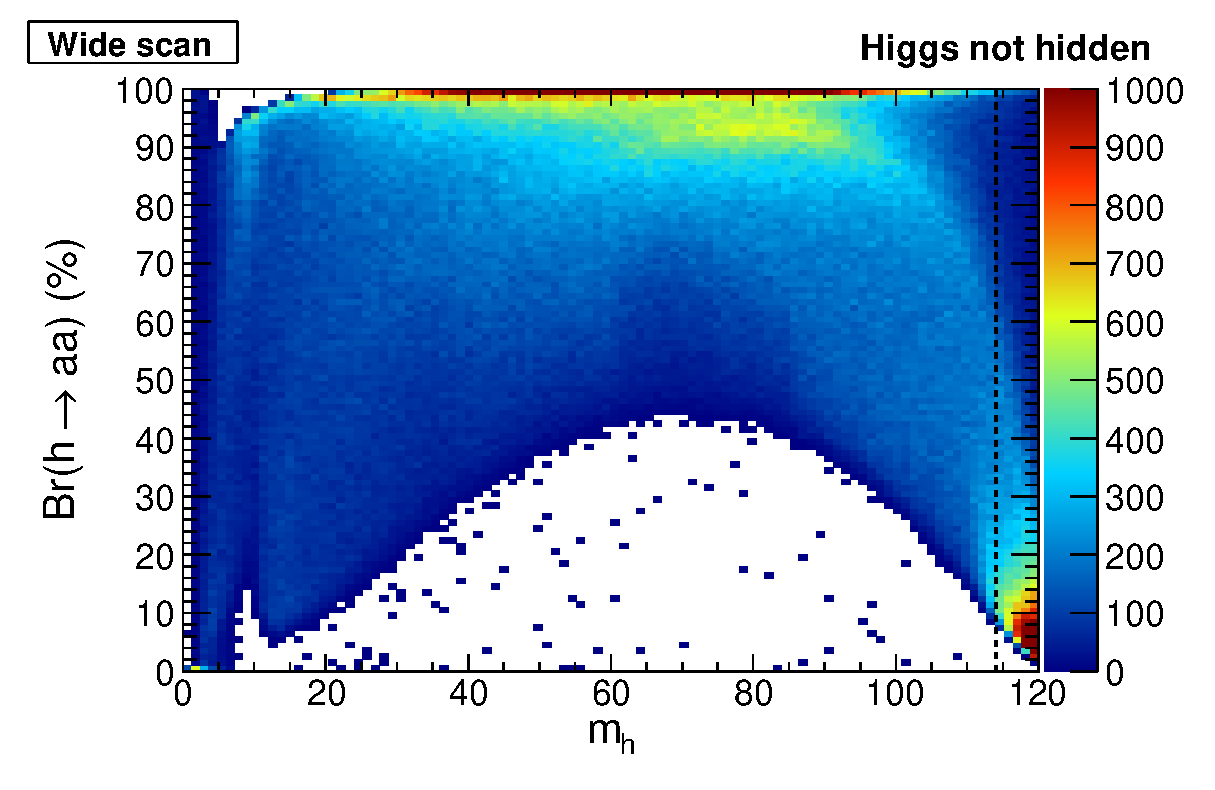
\includegraphics[width=0.5\linewidth]{plots/mh_brhaa.eps}
\caption{Left: regions of $m_a$ vs.\ $m_h$ excluded by LEP searches,
  right: the strong correlation between $m_h$ and $B_{h \to aa}$.  
  The above scan is subject to experimental constraints (other
  than the two specialized LEP searches for $h\to aa$) which require a
  conventionally-decaying Higgs to have $m_h >
  114$~GeV. \label{mass_exclusion}}
\end{center}
\end{figure}


Fig~\ref{pmass1_Akappa} demonstrates the clear correlation between
$m_{a_1}$ and $\lambda$(left)
as well as 
$m_{a_1}$ and $A_{kappa}$(right)
in terms of density of randomly scattered points
({\bf would also good to have plots for $m_{a_1}$ vs $\kappa/\lambda$
     since  $\kappa/\lambda$ is our principle parameter}).
We can see that if the mass of $a_1$ is  below its $\tau$ threshold decay 
then $\lambda$ is confined to be  below 0.1
while $A_\kappa$ is confined to be $|A_\kappa|<0.1$
({\bf Jim, please,  check this statement from the wider scan}).
\begin{figure}[htb]
\begin{center}
\includegraphics[width=0.5\linewidth]{plots/pmass1_lambda.eps}%
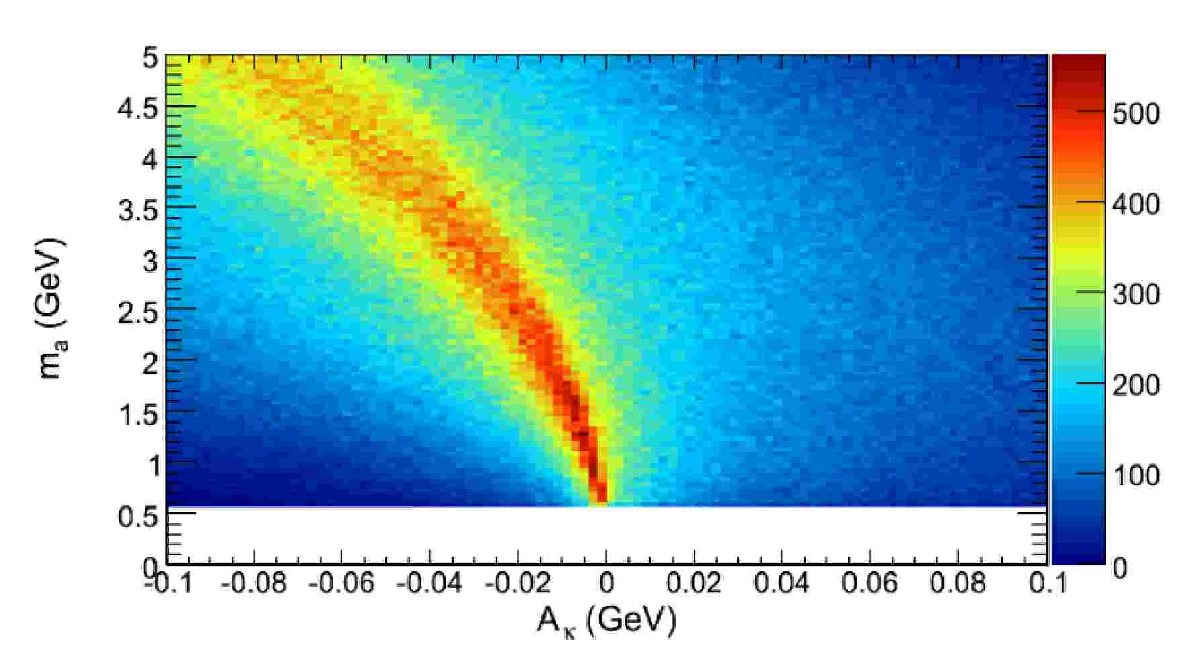
\includegraphics[width=0.5\linewidth]{plots/ma_vs_a-kappa.eps}

\caption{Both $\lambda$ and $A_\kappa$ must be close to zero for $m_a$
  to be below the $2 \, m_\tau$ threshold. \label{pmass1_Akappa}}
\end{center}
\end{figure}

It is also essential to stress that $m_{a_1}<2m_\tau$
condition forces the lightest CP-odd Higgs $a_1$ to be
the singlet with very good accuracy. It's non-singlet admixture is
below 1\%, while for the lightest CP-even Higgs boson, $h_1$
two scenarios can be realized as mentioned above.
In Fig.~\ref{ma-vs-mh-vs-scomp}
we present the distribution of the admixture of the singlet component of  the
$h_1$ in the $m_{a_1}-m_{h_1}$ plane.

\begin{figure}[htb]
\begin{center}
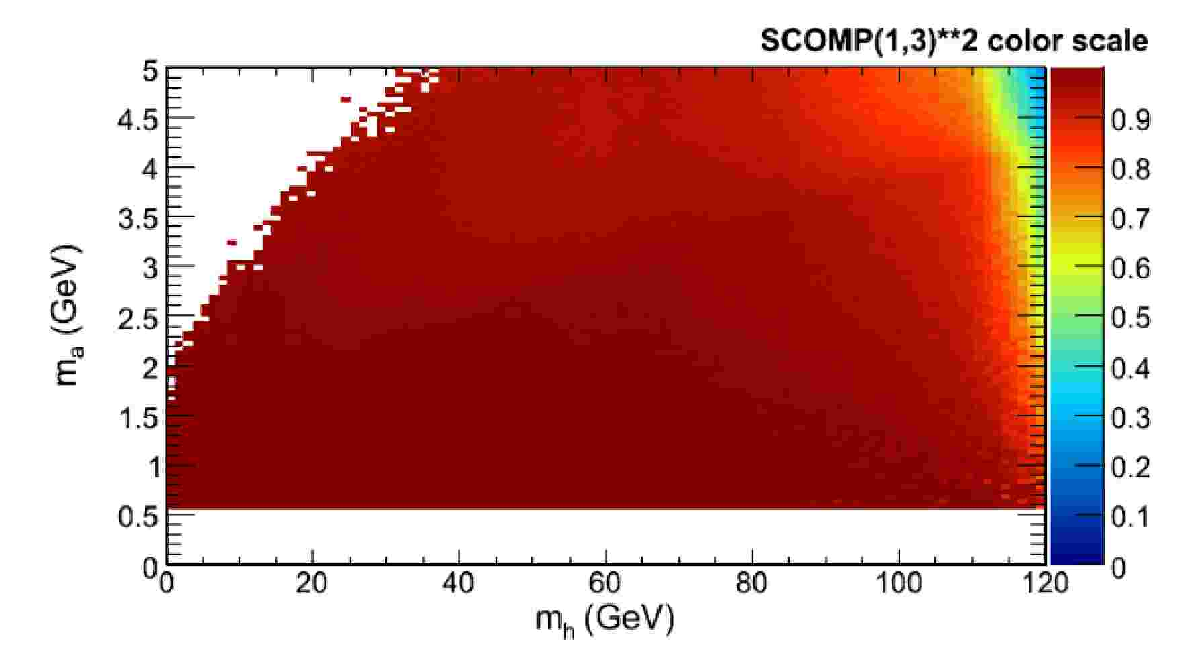
\includegraphics[width=0.75\linewidth]{plots/ma-vs-mh-vs-scomp.eps}
\caption{Distribution of the admixture of the singlet component of  the
$h_1$ in the $m_{a_1}-m_{h_1}$ plane
\label{ma-vs-mh-vs-scomp}}
\end{center}
\end{figure}
One see that singlet component is dominated over the
whole parameter space subject of our scan except the region 
of the $m_{h_1}$ around 120 GeV when $h_1$ is essentially SM-like.
When the $h_1$ is essentially singlet, then role of the SM-like Higgs
is played by the next-to-lightest CP-even Higgs boson, $h_2$.
In Fig.~\ref{mh2-mh1-scomp} we illustrate this
presenting 
singlet and non-singlet admixture of $h_1$
in $m_{h_2}-m_{h_1}$ plane.
\begin{figure}[htb]
\begin{center}
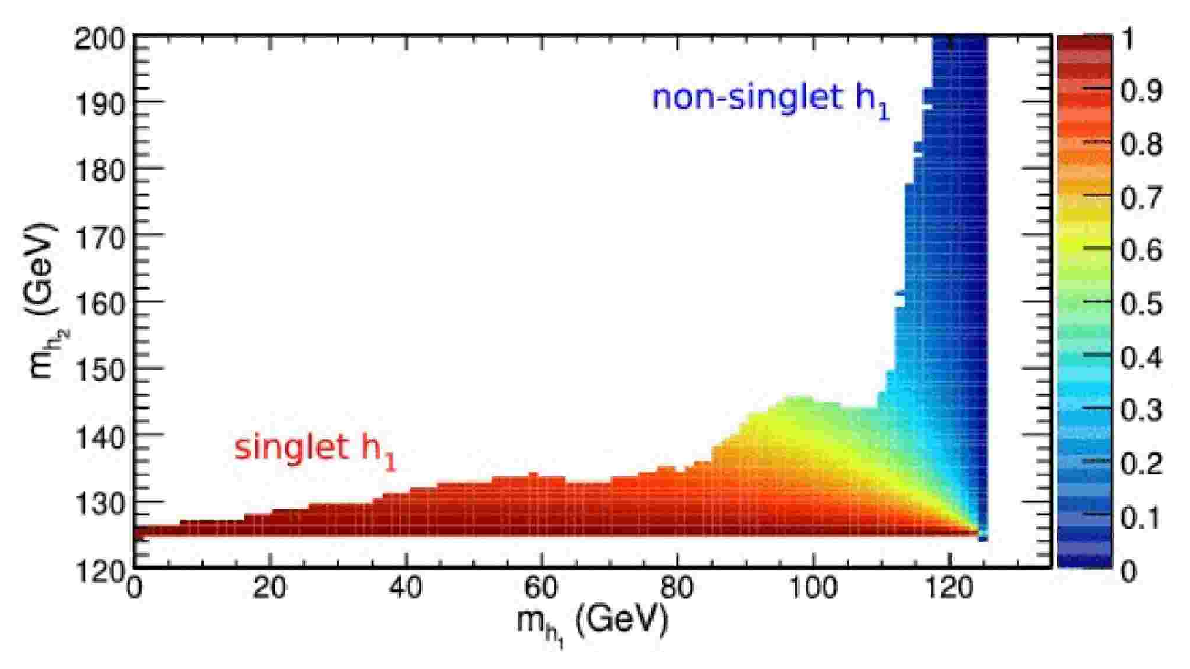
\includegraphics[width=0.75\linewidth]{plots/mh2-mh1-singlet.eps}
\caption{Singlet and non-singlet admixture of $h_1$
in $m_{h_2}-m_{h_1}$ plane
\label{mh2-mh1-scomp}}
\end{center}
\end{figure}

%%%%%%%%%%%%%%%%%%%%%%%%%%%%%%%%%%%%%%%%%%%%%%%%%%%%%%%%%%%%%%%%%%%%%%
%%%%%%%%%%%%%%%%%%%%%%%%%%%%%%%%%%%%%%%%%%%%%%%%%%%%%%%%%%%%%%%%%%%%%%
\subsection{The $h_1$ and $a_1$ branching ratios}

Since $a_1$ is essentially singlet, the singlet admixture
of $h_1$ defines its coupling to $a_1$
and the respective branching ratio $Br(h_1\to a1 a_1)$
as illustrated in Fig.~\ref{scomp13-vs-br-h-aa}
which presents singlet component of $h_1$
(mixing angle squared of the $h_1$ and the pure singlet state,
which is given by \verb|SCOMP(1,3)|$^2$ parameter in NMSSM tools)
versus $Br(h_1\to a1 a_1)$. 

\begin{figure}[htb]
\begin{center}
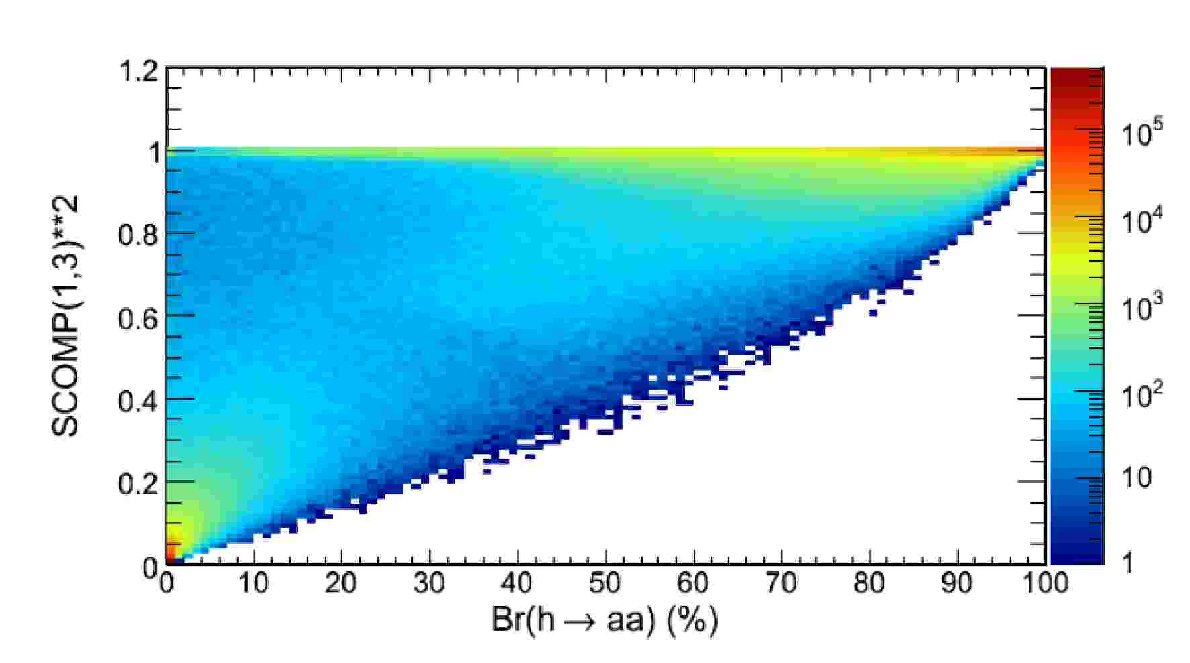
\includegraphics[width=0.75\linewidth]{plots/scomp13_vs_br_h-aa.eps}
\caption{Singlet component of $h_1$
(mixing angle squared of the $h_1$ and the pure singlet state)
versus $Br(h_1\to a1 a_1)$
\label{scomp13-vs-br-h-aa}}
\end{center}
\end{figure}


The essential parameter which controls  the $h_1$ to be a
singlet or non-singlet we have found to be the ratio of
$\kappa/\lambda$  
({\bf I think we need a plot scomp(1,3)$^2$
vs $\kappa/\lambda$  illustrating this}) 
which is eventually
controls  $Br(h_1\to a1 a_1)$ as demonstrated by $Br(h_1\to a1
a_1)$ vs  $\kappa/\lambda$ distribution in
Fig.~\ref{br-h-aa_vs_kap-lam}. One clearly see that for 
$\kappa/\lambda<0.3$, the $Br(h_1\to a1 a_1)$ is significant
which is related to the fact that the singlet component of
$h_1$ is large. One can see that the typical value of  
$Br(h_1\to a1 a_1)$ in this region is 70-100\%. 
({\bf What are
competing Br of $h_1$ in this region?})




\begin{figure}[htb]
\begin{center}
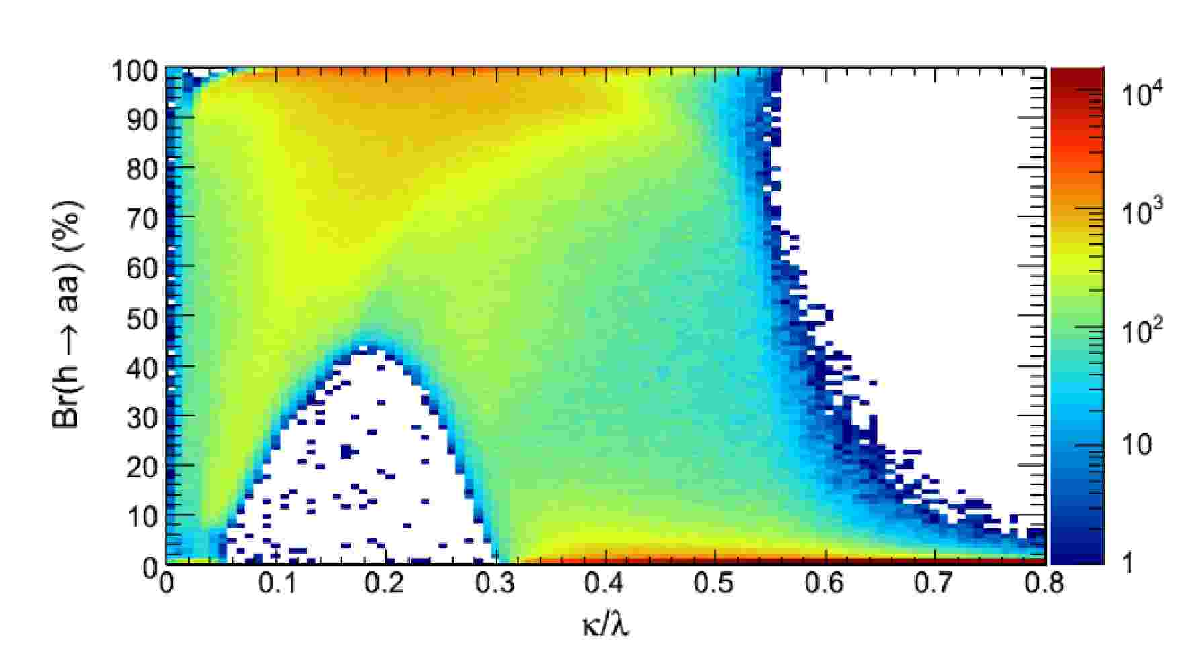
\includegraphics[width=0.75\linewidth]{plots/br-h-aa_vs_kap-lam.eps}
\caption{ $Br(h_1\to a1 a_1)$ vs  $\kappa/\lambda$
distribution.
\label{br-h-aa_vs_kap-lam}}
\end{center}
\end{figure}
The singlet and non-singlet 
features of the lightest CP-even Higgs boson, $h_1$,
can be clearly disentangled in $\mu-\kappa/\lambda$
plane as one can see from Fig.\ref{mu-kaplam-scomp}.
For  $mu\simeq 110$~GeV,
$h_1$
becomes a singlet already for $\kappa/\lambda<0.5$ while for  $mu\simeq 200$~GeV
$h_1$ turns to be a singlet when $\kappa/\lambda<0.3$.
One can clearly see that $\mu$ and $\kappa/\lambda$
are essential variables defining the property of $h_1$
of being  singlet or non-singlet. 
({\bf Why $\mu$ parameter was chosen in this narrow 100-200 GeV
range in our scan?\\
 One more remark/request: since  $\mu$ and $\kappa/\lambda$
 are very important parameters for the $h_1$, I would like to ask you to make
 plot
for the  color map of  $Br(h \to a_1 a_1)$
 in the same, ($\mu$-$\kappa/\lambda$) plane  -- this would be Fig.7b.
 })
\begin{figure}[htb]
\begin{center}
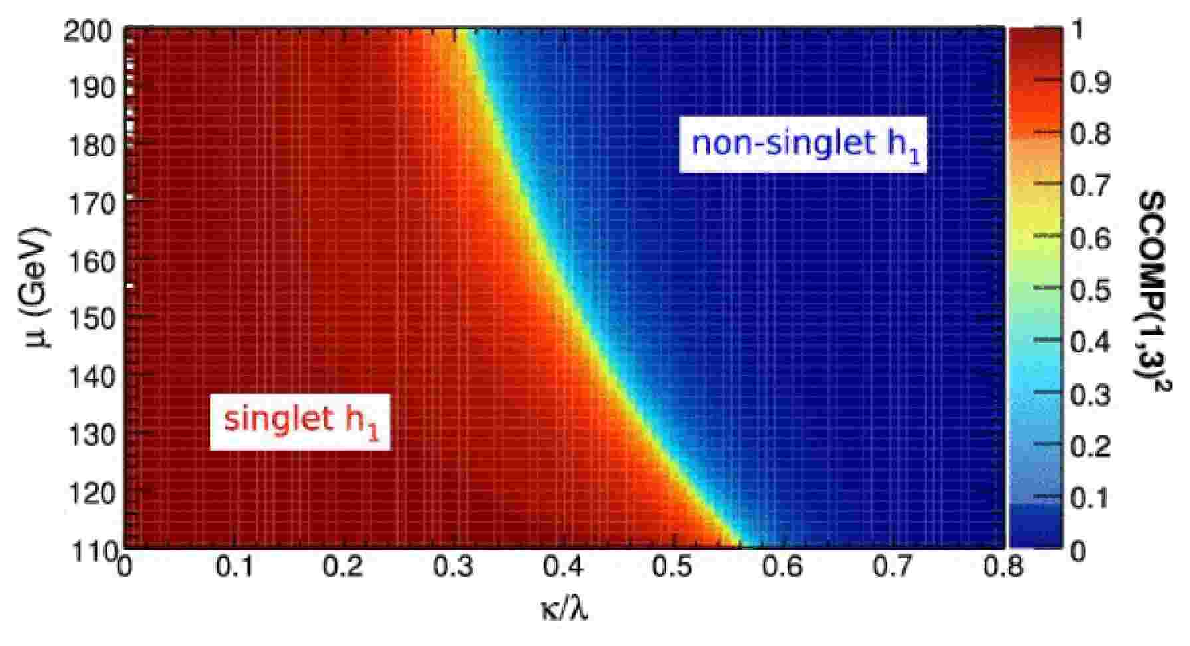
\includegraphics[width=0.75\linewidth]{plots/mu-kaplam-scomp.eps}
\caption{The singlet and non-singlet 
features of the lightest CP-even Higgs boson, $h_1$, 
in $\mu-\kappa/\lambda$
plane.
\label{mu-kaplam-scomp}}
\end{center}
\end{figure}
Another representative plot  separating
singlet and non-singlet $h_1$ states
is the scatter plot of  the partial decay width $\Gamma(h_1\to a_1 a_1)$
versus  $\Gamma(h_1\to jj +bb+WW)$ shown in Fig.\ref{gh1-aa_vs_gh1-conv}.
The red and blue dots here denotes $h_1$ 
being 90\% singlet or 90\% non-singlet respectively.
({\bf Did you include $h_1 \to \tau\tau$ ?})
One can see again how well  singlet/non-singlet states are separated
in the plane of these variables.
\begin{figure}[htb]
\begin{center}
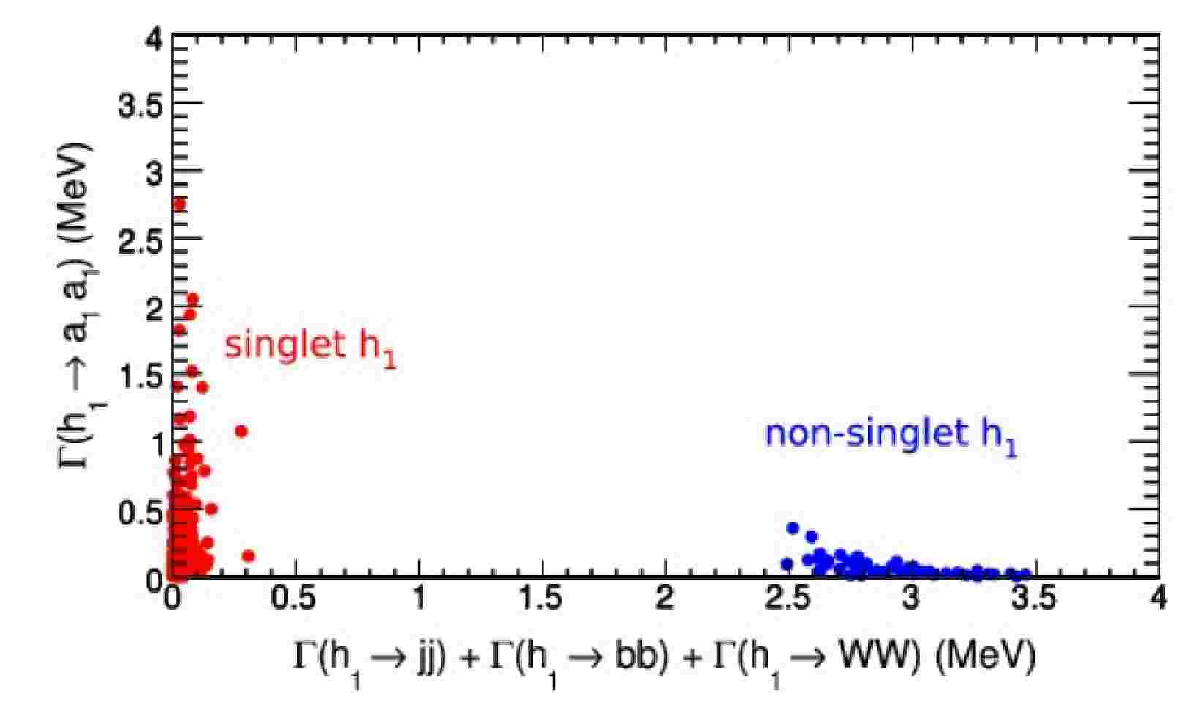
\includegraphics[width=0.75\linewidth]{plots/gh1-aa_vs_gh1-conv.eps}
\caption{Scatter plot of  the partial decay width $\Gamma(h_1\to a_1 a_1)$
versus  $\Gamma(h_1\to jj +bb+WW)$ .
The red and blue dots here denotes here that $h_1$ is
being 90\% singlet or 90\% non-singlet respectively.
\label{gh1-aa_vs_gh1-conv}}
\end{center}
\end{figure}

As we have mentioned above,
$a1$ Higgs boson has extremely small non-singlet 
admixture  in the region of our interest
($m_{a1} < 2m_\tau$),  however even though its non-singlet component is very smaill,
its branching ratio to $\mu^+\mu^-$ is large as soon as 
it kinematically allowed.
In Fig.\ref{pcomp13_vs_br_a-mm} (left) we present how large the  singlet
component of the light  $a_1$ can be  versus $Br(a_1\to\mu\mu)$.
In the Fig.\ref{pcomp13_vs_br_a-mm} (right) we show $m_{a1}$ distribution
in $\lambda-A_\kappa$ plain together with contour of the maximum value of 
$Br(a1\to \mu\mu)$ which is reached by at $m_{a1}\simeq 2$~GeV.
({\bf I wanted to ask Jim the question about the meaning of the color.
     This point  should be clearly explained from the very beginning,
     when we start presenting plots like these.
     The question is the following: for each point(small area) in $\lambda-A_\kappa$
     plain we can have different values of $m_{a1}$. So, for the plot do you chose
     the max or min value of the  $m_{a1}$ for the color map?\\
     Another remark: eventually the left figure should be replotted in more 
     sensible way} )

\begin{figure}[htb]
\begin{center}
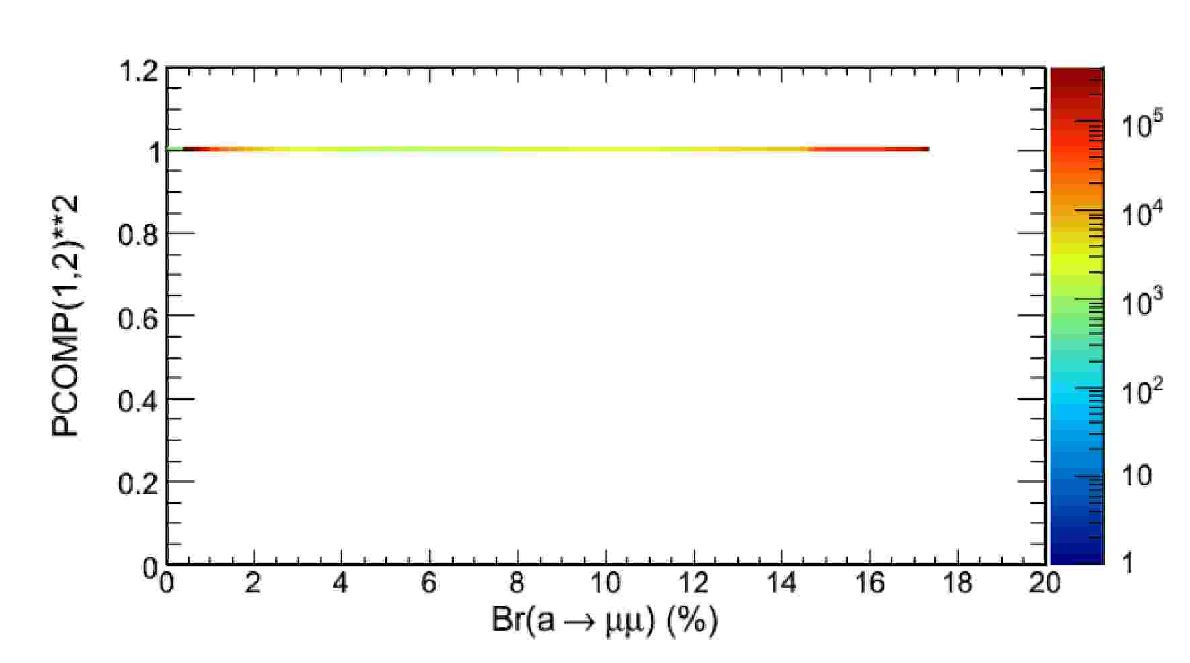
\includegraphics[width=0.5\linewidth]{plots/pcomp13_vs_br_a-mm.eps}%
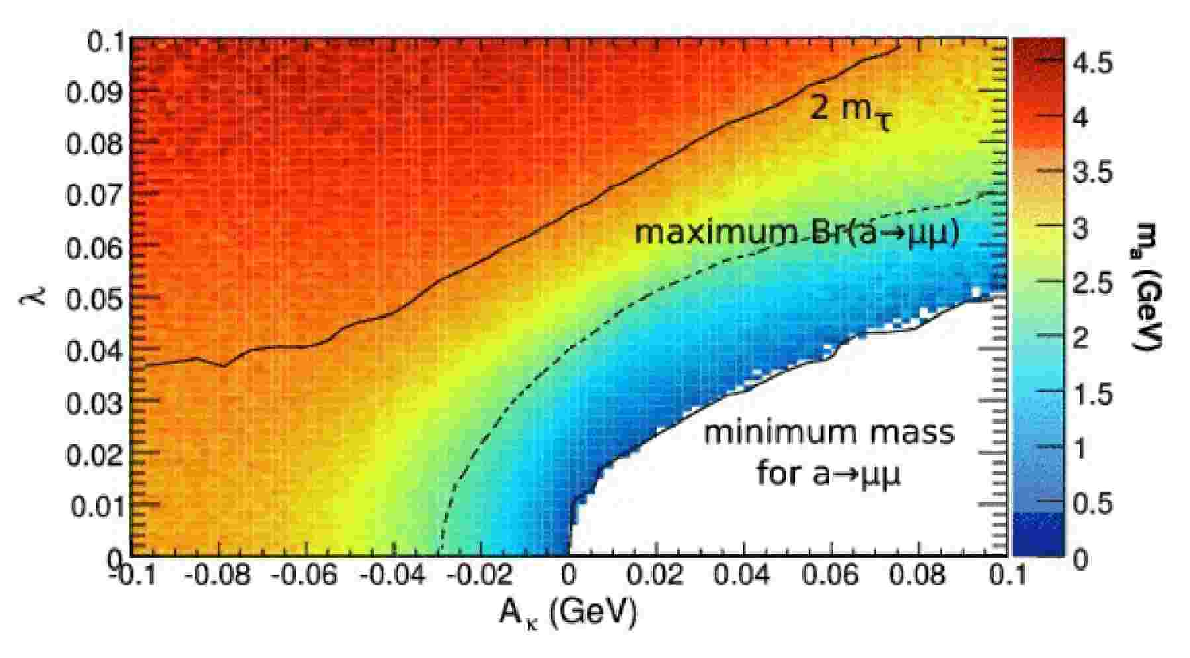
\includegraphics[width=0.5\linewidth]{plots/lam_vs_akap_ma.eps}
\caption{Left: the value of  singlet
component of the light  $a_1$ is versus $Br(a_1\to\mu\mu)$.
Right: $m_{a1}$ distribution
in $\lambda-A_\kappa$ plain together with contour of the maximum value of
$Br(a1\to \mu\mu)$ (dashed contour) 
which depends only on the kinematics defined by the $m_{a1}$.
\label{pcomp13_vs_br_a-mm}}
\end{center}
\end{figure}

In Fig.~\ref{br-h-aa_vs_ma} we present the  value 
of  $Br(a_1\to\mu\mu)$ versus $m_{a1}$ which
we have tabulated and use in our analysis. 
It is important to stress that for a given $m_{a1}$
the value of  $Br(a_1\to\mu\mu)$ is essentially fixed
and is practically independent off other model parameters.
({\bf We need more details on 
how this  Br is independent off other parameters
and how large deviations 
from the red curve can be. We should probably have
one more additional figure on this}).
\begin{figure}[htb]
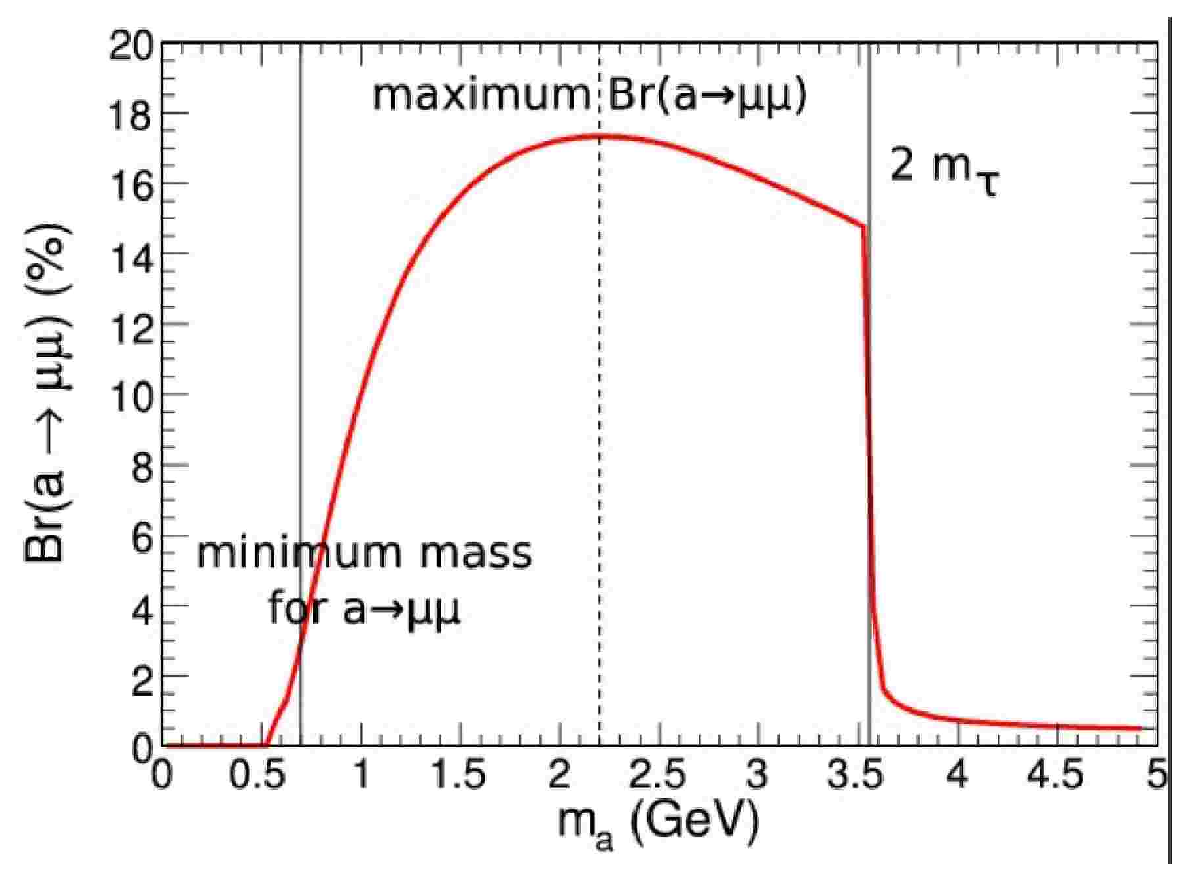
\includegraphics[width=0.75\linewidth]{plots/br-h-aa_vs_ma.eps}%
\caption{The  value 
of maximal  $Br(a_1\to\mu\mu)$ versus $m_{a1}$ 
\label{br-h-aa_vs_ma}}
\end{figure}
We can see that $Br(a_1\to\mu\mu)$ can be as large as 18\%
for $m_{a1}$ around 2 GeV.
In the mass
range of interest (below the $a \to \tau^+\tau^-$ threshold), the main
competing channels are $a \to gg$ and $a \to s\bar{s}$.


%%%%%%%%%%%%%%%%%%%%%%%%%%%%%%%%%%%%%%%%%%%%%%%%%%%%%%%%%%%%%%%%%%%%%%
%%%%%%%%%%%%%%%%%%%%%%%%%%%%%%%%%%%%%%%%%%%%%%%%%%%%%%%%%%%%%%%%%%%%%%
\subsection{Production rates}

As we have shown,
the lightest CP-even Higgs boson, $h_1$,
typically has significant singlet component
in the region of our  interest 
(i.e. in the region of $m_{a1}<2 m_{\tau}$) 
and as we have found above,
both, $Br(h_1\to a_1 a_1)$  and $Br(a_1\to \mu\mu)$,
are quite significant. In the same time,
one should expect the suppression
of the $h_1$ production rate since $h_1$ interacts weakly with the 
fermions and gauge bosons  due to its  singlet nature.

In our study we have evaluated $pp\to h_1$ production cross section
for the $gg\to h_1$ and $b\bar{b}\to h_1$ process
at the next-to-leading order (NLO)
using the following 
procedure.

First, we have used  
HIGLU v2.102 package~\cite{Spira:1995rr} to calculate 
SM Higgs production cross section in $gg\to H_{SM}$ process.
Since the ratio of  $\sigma(gg\to h_1)/\sigma(gg\to H_{SM})$
production cross sections is equal to the ratio
of partial decay widths $\Gamma(h_1\to gg)/\Gamma(H_{SM}\to gg)$, one finds
\begin{equation}
\sigma(gg\to h_1)=\sigma(gg\to H_{SM})\frac{\Gamma(h_1\to gg)}{\Gamma(H_{SM}\to gg)}
=\sigma(gg\to H_{SM})\frac{Br(h_1\to gg)\Gamma^{tot}(h_1)}{\Gamma(H_{SM}\to gg)}.
\end{equation}
Therefore we have all components to evaluate $\sigma(gg\to h_1)$:
we use
$\sigma(gg\to H_{SM})$ and $\Gamma(H_{SM}\to gg)$ calculated  using HIGLU at  NLO,
while $Br(h_1\to gg)$ and $\Gamma^{tot}(h_1)$ we obtain using NMSSMtools.


\begin{figure}[htb]
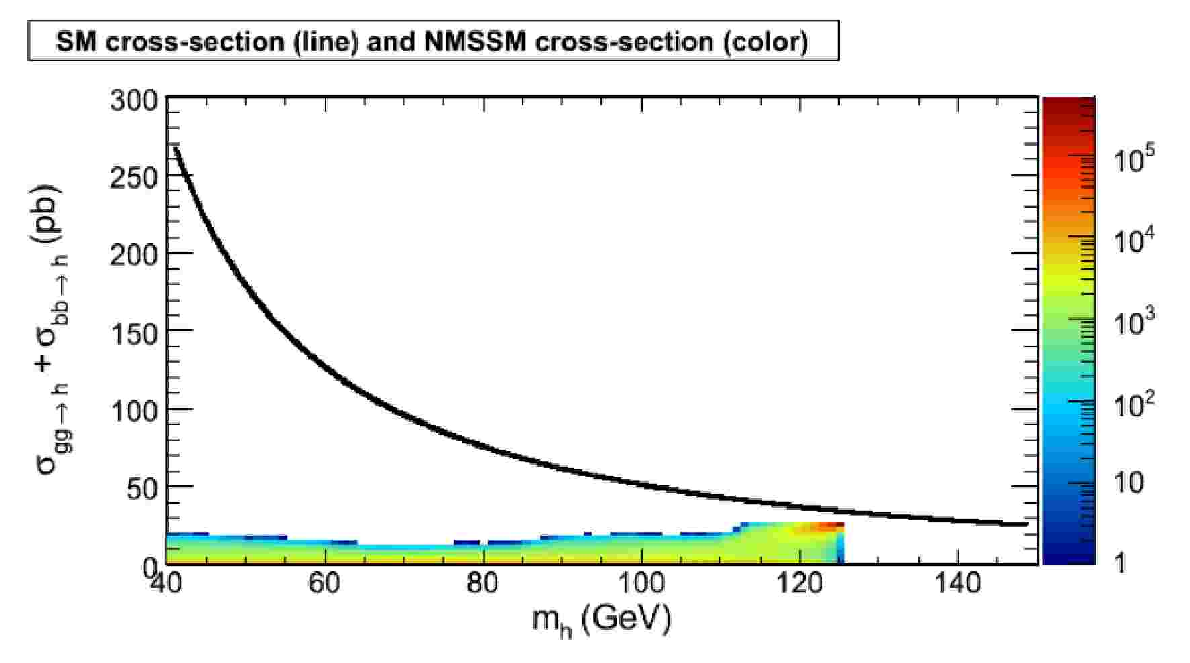
\includegraphics[width=0.5\linewidth]{plots/cs3.eps}%
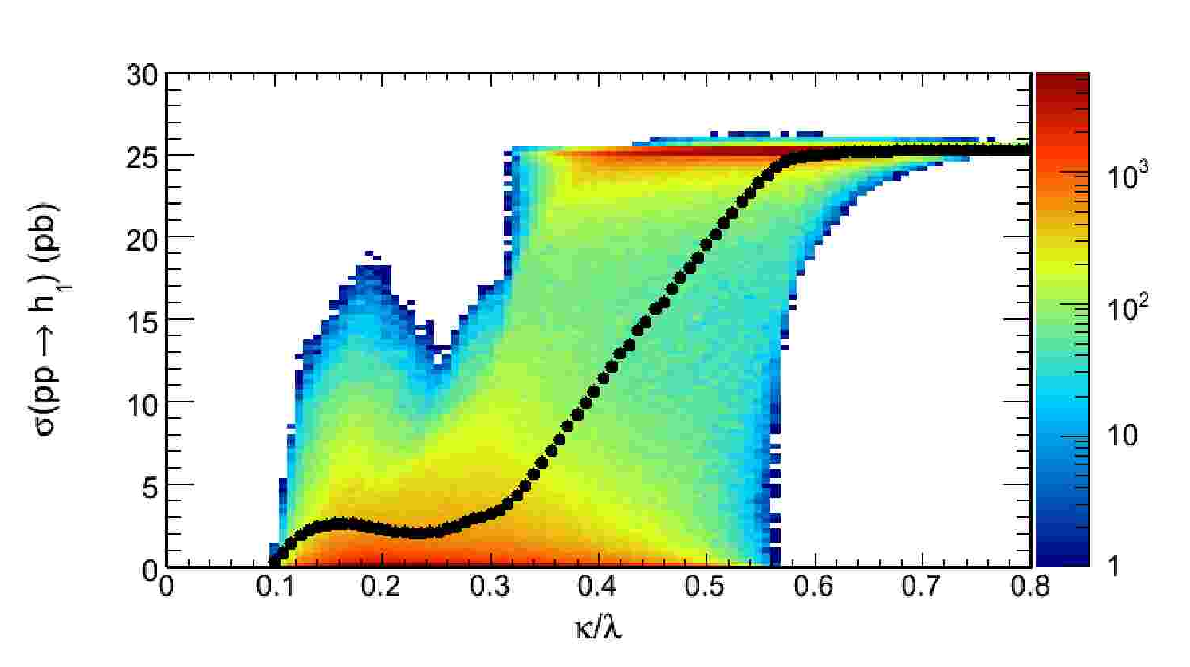
\includegraphics[width=0.5\linewidth]{plots/sig_vs_kaplam.eps}%
\caption{Combined 
$\sigma(gg\to {\cal H}) + \sigma(b\bar{b}\to {\cal H})$ production cross section
versus $m_{\cal H}$ for NMSSM and SM,
where ${\cal H}$ stands either for NMSSM or SM Higgs boson.
\label{cs3}}
\end{figure}

The cross section of $b\bar{b}\to h_1$ was also evaluated at
NLO as follows. The numerical calculation for the  SM Higgs
production in  $b\bar{b}\to H_{SM}$ fusion has been carried out
with the program developed in \cite{Balazs:1998sb} and lately
used also in \cite{Belyaev:2005nu} where the QCD-improved
(running) Yukawa couplings have been used. Then using
$Y_{bbh_1}/Y_{bbH_{SM}}$ ratio of  Yukawa couplings 
calculated  in NMSSMtools, one finds:
\begin{equation}
\sigma(b\bar{b}\to h_1)=\sigma(b\bar{b}\to H_{SM})
\left(\frac{Y_{bbh_1}}{Y_{bbH_{SM}}}\right)^2
\end{equation}
For the evaluation of production cross sections, CTEQ6M set for
parton density function set was used. 

Our first results  on the
combined  $\sigma(gg\to {\cal H}) + \sigma(b\bar{b}\to {\cal
H})$ production cross section versus $m_{\cal H}$ for NMSSM and
SM  are presented in Fig.\ref{cs3} (left), where ${\cal H}$ stands
either for NMSSM or SM Higgs boson. 
The right frame of Fig.\ref{cs3} 
presents $\sigma(gg\to {\cal H}) + \sigma(b\bar{b}\to {\cal
H})$ versus $\kappa/\lambda$ for NMSSM in more details. 
({\bf Can we present(or
think about how to present) also results for $\sigma(gg\to
{\cal H})$ $\sigma(b\bar{b}\to {\cal H})$ separately to show
their relative contribution? }).
From Fig.~\ref{cs3} we can see that 
production cross section of NMSSM $h_1$ is indeed
suppressed typically by 2 orders of magnitude as compared to the
SM Higgs boson production in case when 
$h_1$ has a significant singlet component. The value of the
minimal suppression depends on the mass of $h_1$:
for $m_{h1}\simeq 40-50$ GeV, the maximal cross section of $h_1$
production is about 10 smaller than the SM one, while
when  $m_{h1}\simeq 115-125$ GeV its production cross section
is quite close to SM and can be as large as about 25 pb 
once the singlet component of $h_1$
vanishes.

Since we study the whole production and decay chain
$pp\to h_1 \to a_1 a_1\to 4\mu$ let us  look at the
cross section of the four-muon production after application
of the respective branching ratios from NMMStoos
to the $h_1$ production cross section which we have evaluated.

\begin{figure}[h]
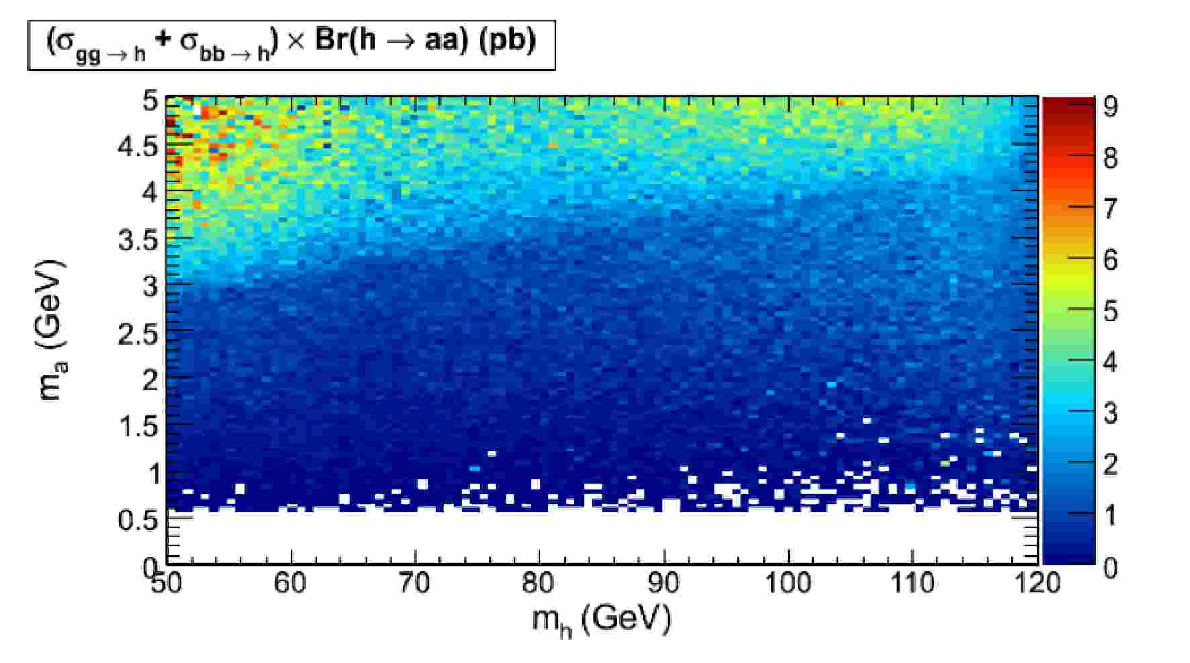
\includegraphics[width=0.5\linewidth]{plots/cs1.eps}%
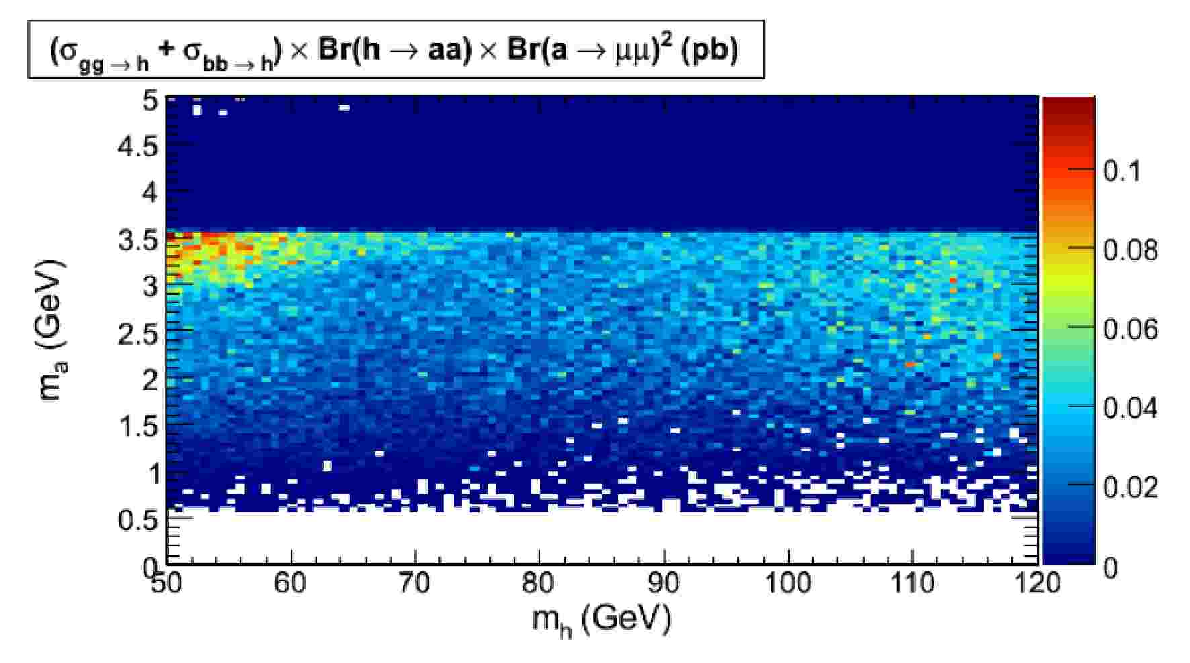
\includegraphics[width=0.5\linewidth]{plots/cs2.eps}%
\caption{$m_{a1}-m_{h1}$ plane with
color map distribution of
for $\sigma(gg+b\bar{b}\to h_1)\times Br(h_1\to a_1 a_1)$ (left) 
and $\sigma(gg+b\bar{b}\to h_1)\times Br(h_1\to a_1 a_1)
\times Br(a_1\to \mu\mu)^2$ (right) rates.
\label{cs2}}
\end{figure}
\begin{figure}[h]
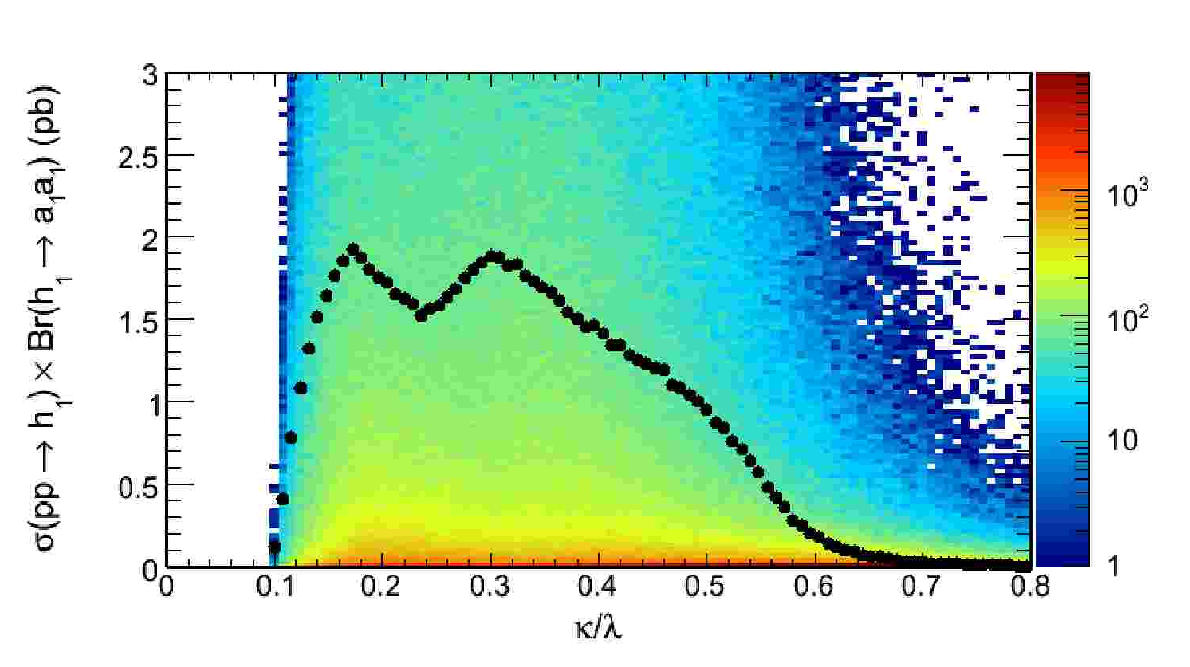
\includegraphics[width=0.5\linewidth]{plots/sig-brh2a_vs_kaplam.eps}%
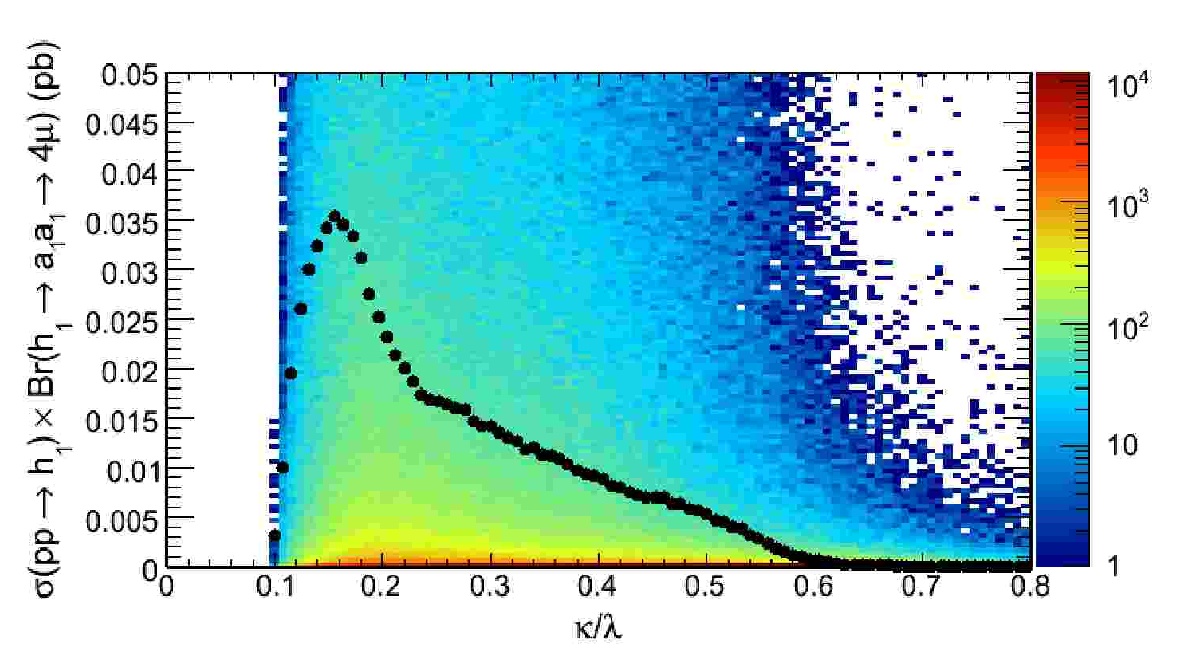
\includegraphics[width=0.5\linewidth]{plots/sig-brh2a-bra2mu_vs_kaplam.eps}%
\caption{
Distribution of
$\sigma(gg+b\bar{b}\to h_1)\times Br(h_1\to a_1 a_1)$ (left)
and 
$\sigma(gg+b\bar{b}\to h_1)\times Br(h_1\to a_1 a_1)
\times Br(a_1\to \mu\mu)^2$ (right) (right)
rates
versus  $\kappa/\lambda$.
\label{sig-brh2a_vs_kaplam}}
\end{figure}

In Fig.\ref{cs2} we present $m_{a1}-m_{h1}$ plane with
color map distribution of
for $\sigma(gg+b\bar{b}\to h_1)\times Br(h_1\to a_1 a_1)$ (left) 
and $\sigma(gg+b\bar{b}\to h_1)\times Br(h_1\to a_1 a_1)
\times Br(a_1\to \mu\mu)^2$ (right) rates. One can see that
$\sigma(gg+b\bar{b}\to h_1)\times Br(h_1\to a_1 a_1)$
rate can be quite large and reach about 10 pb for the light $m_{h1}$
with the mass about 50 GeV.
In the same time,
the final cross section of the process under study ---
$\sigma(gg+b\bar{b}\to h_1)\times Br(h_1\to a_1 a_1)
\times Br(a_1\to \mu\mu)^2 \equiv 
\sigma(gg+b\bar{b}\to h_1 \to a_1 a_1 \to 4\mu)$ ---
can be only as large as about 0.1 pb.
In Fig.\ref{sig-brh2a_vs_kaplam}
we present details on the distribution of
$\sigma(gg+b\bar{b}\to h_1)\times Br(h_1\to a_1 a_1)$ (left)
and 
$\sigma(gg+b\bar{b}\to h_1)\times Br(h_1\to a_1 a_1)
\times Br(a_1\to \mu\mu)^2$ (right) (right)
rates
versus  $\kappa/\lambda$.


Even though the four-muon signal rates from NMSSM are not high,
due to relatively low expected backgrounds the signature of our interest
would allow us to exclude significant portion of NMSSM parameter space 
even  at low integrated luminosities as we present below.

The parameter space accessible at the LHC at low and later on at high luminosity regime
is quite unique since it can not be excluded
by present low-energy experiments on rare B-meson decays since, as we have found
the singlet component of the lightest CP-odd Higgs boson, $a_1$,
is extremely close to unity.
({\bf Please  add here reference to the  paper and the talks!}).
\\
\\
({\bf We should note that of course Tevatron is quite competitve with LHC
on the search of $4\mu$ signature from NMSSM since
the production corss section at Tevatron is quite large.
This is related to the fact that we study the system with comparatively small
invariant mass which is not suppressed by gluon parton density
since x-values are not large.
On the other hand we should present a full potential of the LHC
on covering the parameter space of $4\mu$ signature from NMSSM 
down to high luminosity and compare Tevatron and LHC potentials
in the Figure below.})
\begin{figure}[h]
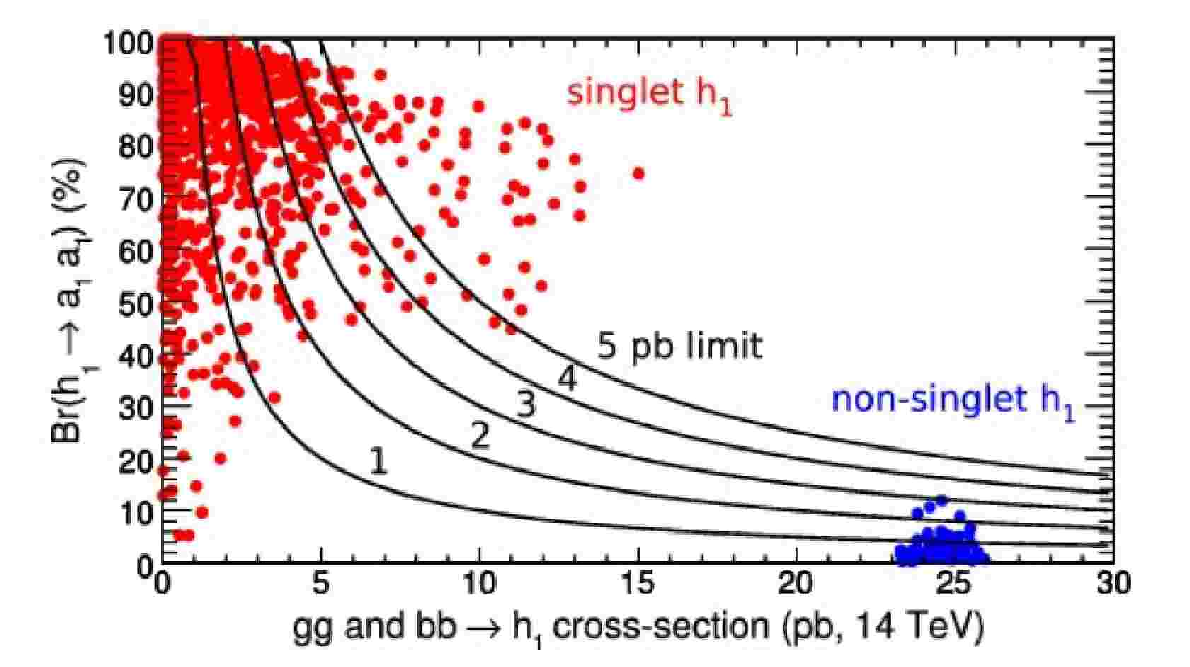
\includegraphics[width=0.5\linewidth]{plots/br_vs_cs.eps}%
\caption{
\label{}}
\end{figure}
({\bf Another point we should probably explore is to add 
     $h2\to h_1 h_1 \to a_1 a_1 + X$ signature. Let me know if you need input from me on this
     subject. We have all ingredients for the production rate, so we can easily add this cahnnel.
     We can add it in this section or later on.
     })
     




\section{Analysis}

The main characteristic of the signal is two back-to-back di-muon pairs with pair consisting of 
spatially close muons. The di-muon pairs should have invariant masses consistent with each, which
serve as a measurement of $m_a$, and the four muon invariant mass distributionshould have a spike 
that corresponding to the $m_h$ mass. We use these striking features of signal events in designing 
the analysis with a reasonably high acceptance and very low backgrounds suitable for early LHC running.

\subsection{Signal Simulation}
We use Pythia to generate signal event templates with $m_h$ in the range from 70 to 140 GeV/c$^2$
and $m_a$  in the range from 0.5 to 4 GeV/c$^2$). For detector response emulation, we chose the CMS 
detector as a benchmark and used its parameters descibed in CMS Technical Design Report. The key 
parameters important for this analysis are muon momentum resolution, low threshold on muons to 
reach the muon system, acceptance and average muon reconstruction efficiencies. {\bf we should quote 
the numbers.} 

\subsection{Event Reconstruction}
The analysis starts by requiring at least four muon candidates with $p_T>5$ \gevc in the fiducial volume of the
detector. At least one of the four muons has to have $p_T>20$ $\gevc$ to suppress major backgrounds and to 
satisfy trigger requirements. Each event must have at least two muon candidates of positive and negative 
charge each. In events satisfying these critiria, we define quadruplets of candidates consisting of two 
positive and two negatively charged muon candidates. Although very unlikely, there can be more than one 
quadruplet per event, e.g. if there are five muons in the event. Each such quadruplet if preserved until the
end of the analysis.

Next, we sort the four muon candidates in quadruplet into two di-muon pairs. We minimize the quantity 
$(\Delta R(\mu_i,\mu_j)^2 + \Delta R (\mu_k,\mu_l)^2)$ under the constarint that each di-muon pair
consists of two muon candidates of opposite charge. We discard quadruplets in which $\Delta R$ between 
muons in any of the two pair exceeds {\bf 0.5???} as this cut is 100\% efficient for the signal while
it can diminish the size of the data sample by removing events, which have topology inconsistent with
signal. At his point in the analysis, the invariant mass of each of the di-muon pair, $m_{12} and m_{34}$, 
is calculated as well as the invariant mass of all four muons, which we denote as $m_{1234}$ or $M$. 
Figure \ref{muon_pairs_masses_invariant_mass}a) shows the invariant mass of the muon pairs passing 
all selections ($m_{12}$ and $m_{34}$ are combined into a single distribution) for two choices of
$m_h$ and $m_a$. Figure \ref{muon_pairs_masses_invariant_mass}b) shows the distribution of the invariant
mass $M$ of the four muon system for two benchmark points. Further background suppression can be
obtained by adding the isolation requirement to one or both di-muon pairs in the event, e.g. by
setting the upper bound on the sum of transverse momenta of all tracks in a cone around the reconstructed
direction of the di-muon pair excluding momenta of the two muon tracks. Such requirement can allow a 
very substantial suppression of the dominant source of the background coming from events with one or more 
muons originating from jets. We choose not to use this critirea as our estimates show that the final rate 
of such background events is already very low. If data shows larger contribution of these events, 
this isolation requirement would allow bringing backgrounds back to very low level at a moderate
cost to signal acceptance.

\begin{figure}[htb]
\begin{center}
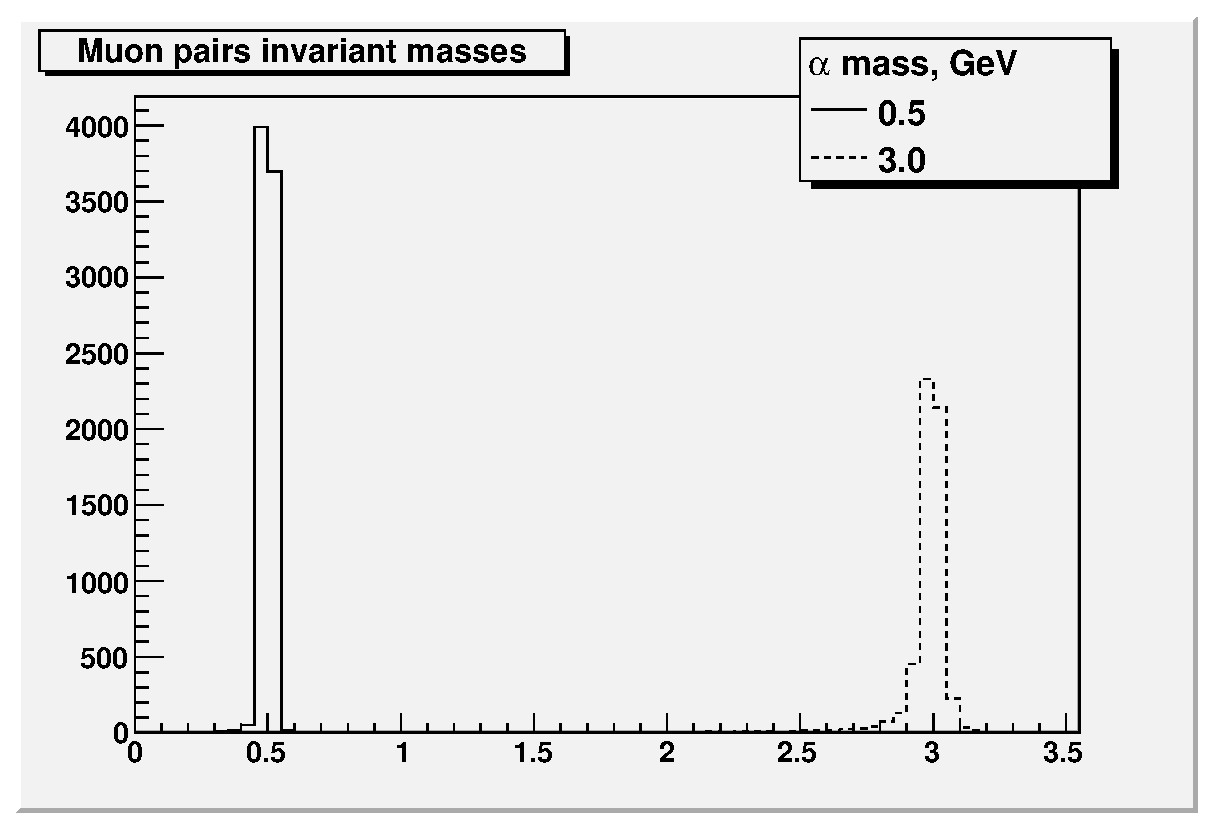
\includegraphics[width=0.48\linewidth]{plots/muon_pairs_masses.eps}
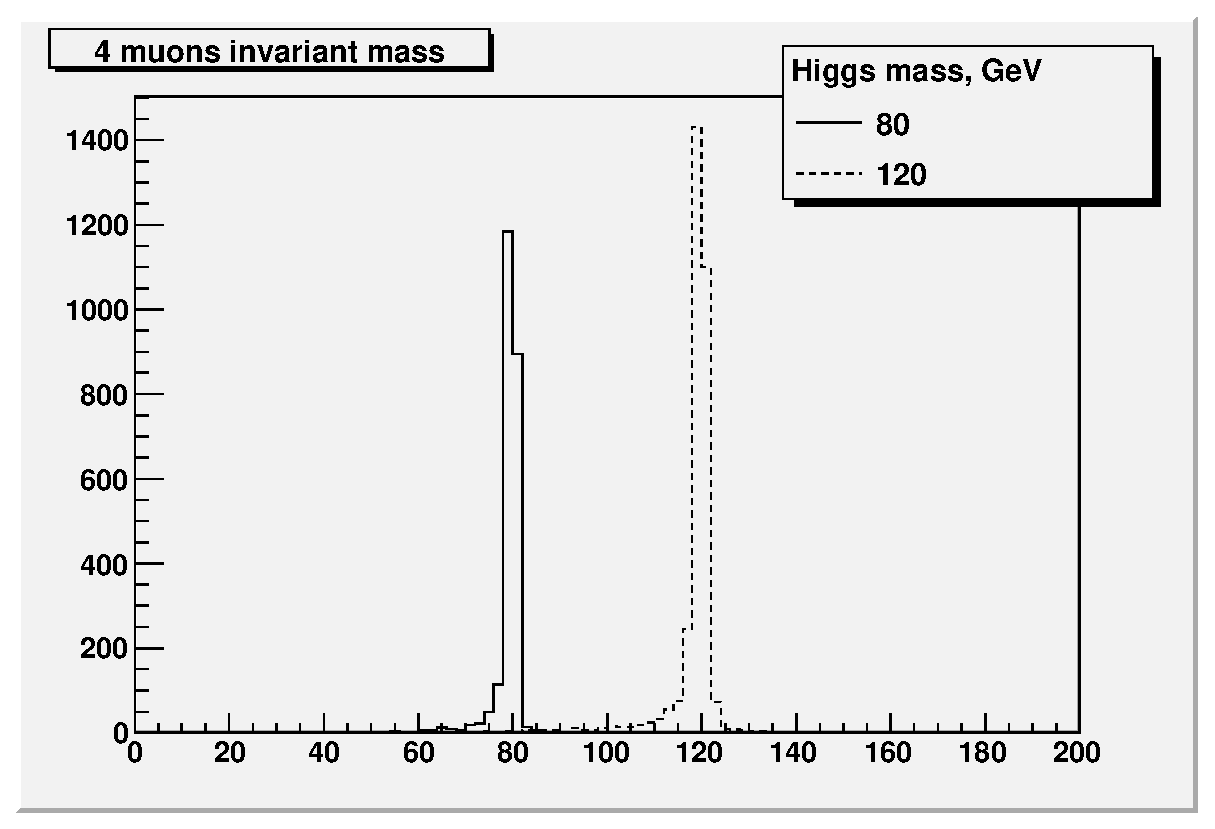
\includegraphics[width=0.48\linewidth]{plots/invariant_mass.eps}
\caption{Left: Reconstructed invariant mass of reconstructed muon pairs for $m_a=0.5$ and 3 GeV/c$^2$ (in both cases $m_H$ = 100 GeV/c$^2$). Right: Reconstructed invariant of four muons for $m_H=80$ and $m_H=120$ GeV/c$^2$ (in both cases $m_a$ = 3.0 GeV).}
\label{muon_pairs_masses_invariant_mass}
\end{center}
\end{figure}

Acceptance of the selections listed above is shown in Table \ref{acceptance} and is large thanks to
the high coverage of the CMS muon system. Figures \ref{signal_acceptance}a) and 
\ref{signal_acceptance}b) illustrate the dependence of acceptance on values of $m_h$ and $m_a$. 

\begin{table}[t]
\caption{Acceptances for various points in $m_h$-$m_a$ space.\label{acceptance}}
\begin{center}
\begin{tabular}{|c|c|c|c|c|c|}
\hline
%\multicolumn{3}{|c|}{hey}\\ \hline
$m_h$, $m_a$ (GeV) & 0.5 & 1.0 &2.0&3.0&4.0\\ \hline
80&    $0.3052\pm0.0046$    &    $0.2656\pm0.0044$    &    $0.2420\pm0.0043$    &    $0.2389\pm0.0043$    &    $0.2324\pm0.0043$    \\ \hline
100&   $0.3915\pm0.0049$    &    $0.3245\pm0.0047$    &    $0.2906\pm0.0045$    &    $0.2862\pm0.0045$    &    $0.2819\pm0.0045$    \\ \hline
120&   $0.4587\pm0.0050$    &    $0.3785\pm0.0049$    &    $0.3405\pm0.0047$    &    $0.3226\pm0.0047$    &    $0.3103\pm0.0046$    \\ \hline
\end{tabular}
\end{center}
\end{table}

\begin{figure}[htb]
\begin{center}
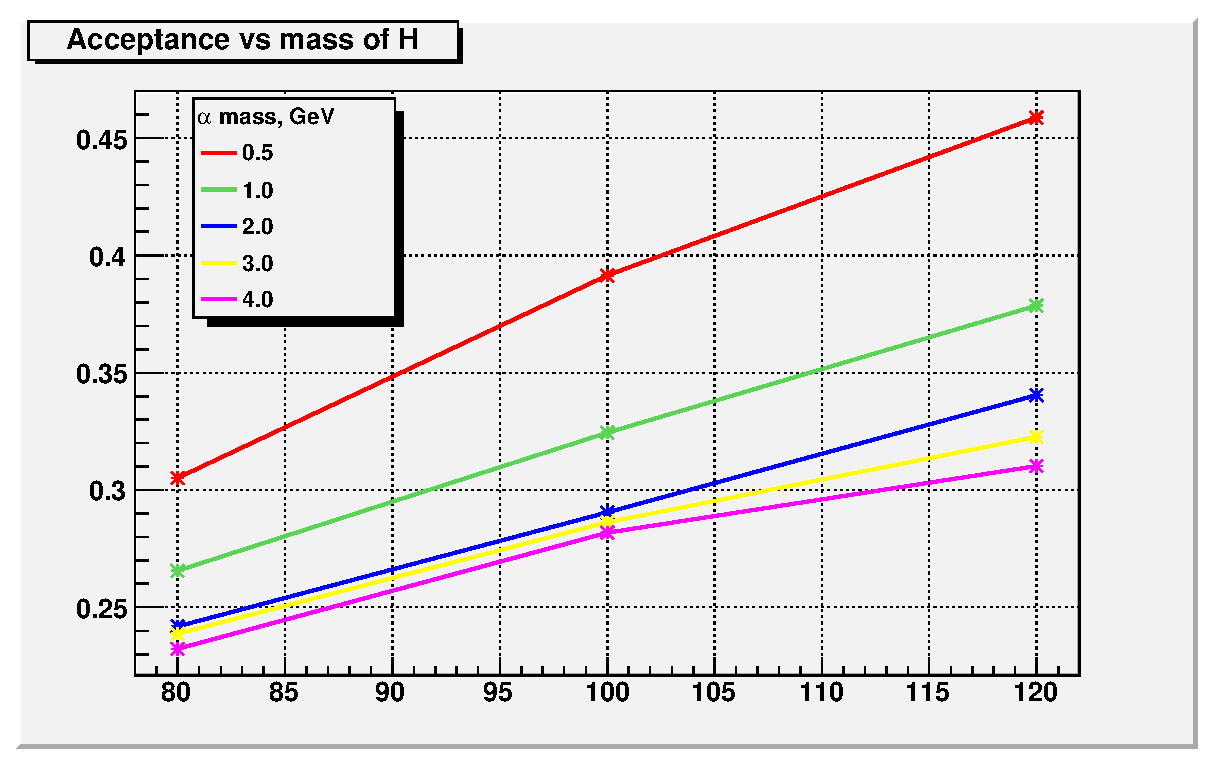
\includegraphics[width=0.48\linewidth]{plots/acceptance_H.eps}
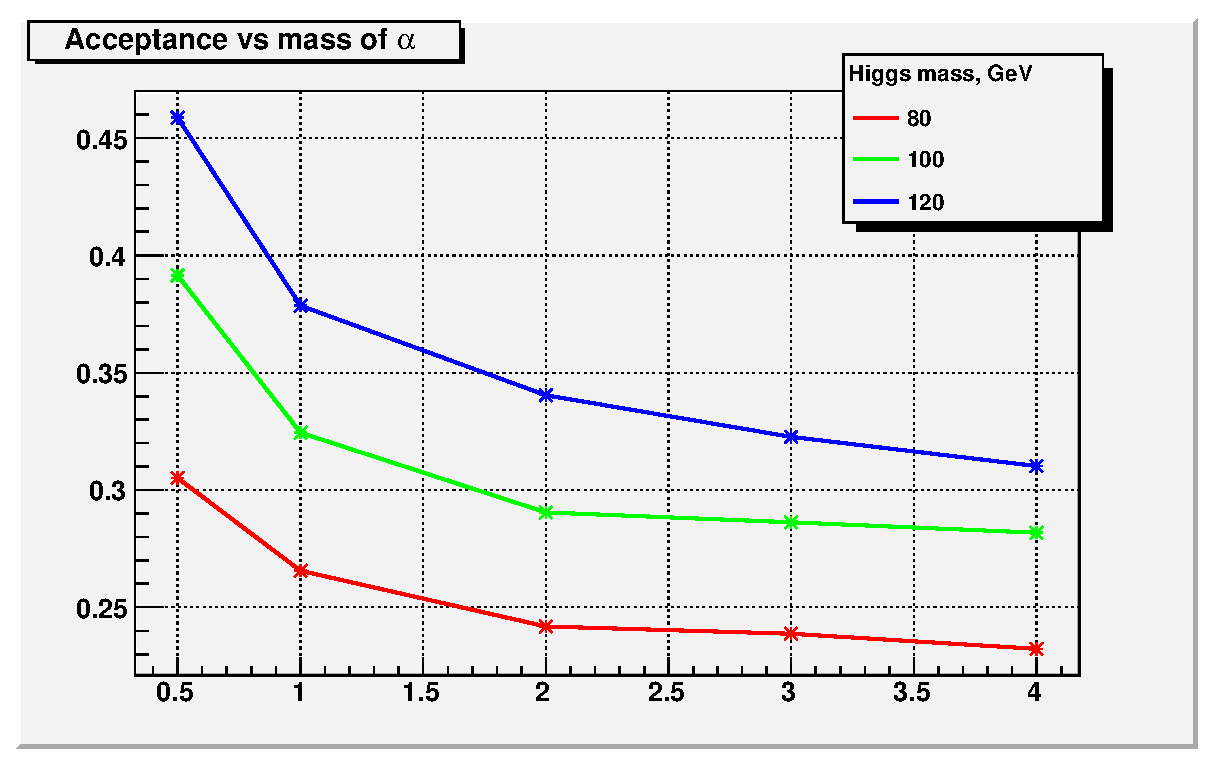
\includegraphics[width=0.48\linewidth]{plots/acceptance_a.eps}
\caption{Acceptance as a function of $m_a$ for fixed $m_h$. Acceptance as a function of $m_h$ for fixed $m_a$.}
\label{signal_acceptance}
\end{center}
\end{figure}

One can further reduce the background events and zoom on the region of interest of
this analysis by applying cuts on $m_{12}$, $m_{34}$, $M$, and require that measured
values of $m_{12}$ and $m_{34}$ are consistent within  uncertainties. Instead of
applying these cuts explicitly, we develop a statistical procedure that performs a fit
in  a 3D space of measured values of $(m_{12},m_{34}, m_{1234})$ taking into account
kinematical properties of  signal events. This approach allows maximizing signal
acceptance and therefore statistical power of the analysis and is discussed in what
follows. It is also convenient from experimental point of view as the backgrounds
will  be distributed in some smooth fashion over the 3D space allowing fitting the 3D
distribution to estimate  backgrounds directly from the data. Potential signal would
appear as a concentration of events in one specific  region in the 3D space (a 3D
``bump''). Figure \ref{muon_pairs_masses_diff} shows the difference in the 
reconstructed masses of the two di-muon pairs in signal events, which determines the
size of the signal region  in the ($m_{12}, m_{34}$) plane.

To give the reader a better idea on the signal significance of this analysis, we quote
efficiencies and  background contamination (next section) for a set of cuts that zooms
on the highest significance region.  The cuts we use are $M>60$ \gevcc, $m_{12} < 4$,
$m_{34} < 4$, and $|m_{12}-m_{34}|<0.08+0.005*(m_{12}+m_{34})$.  The latter cut is
enforcing the requirement that the two pair masses are consistent with each other and 
takes into account widening of the absolute resolution in the reconstructed di-muon
mass as a function of mass. 

\begin{figure}[htb]
\begin{center}
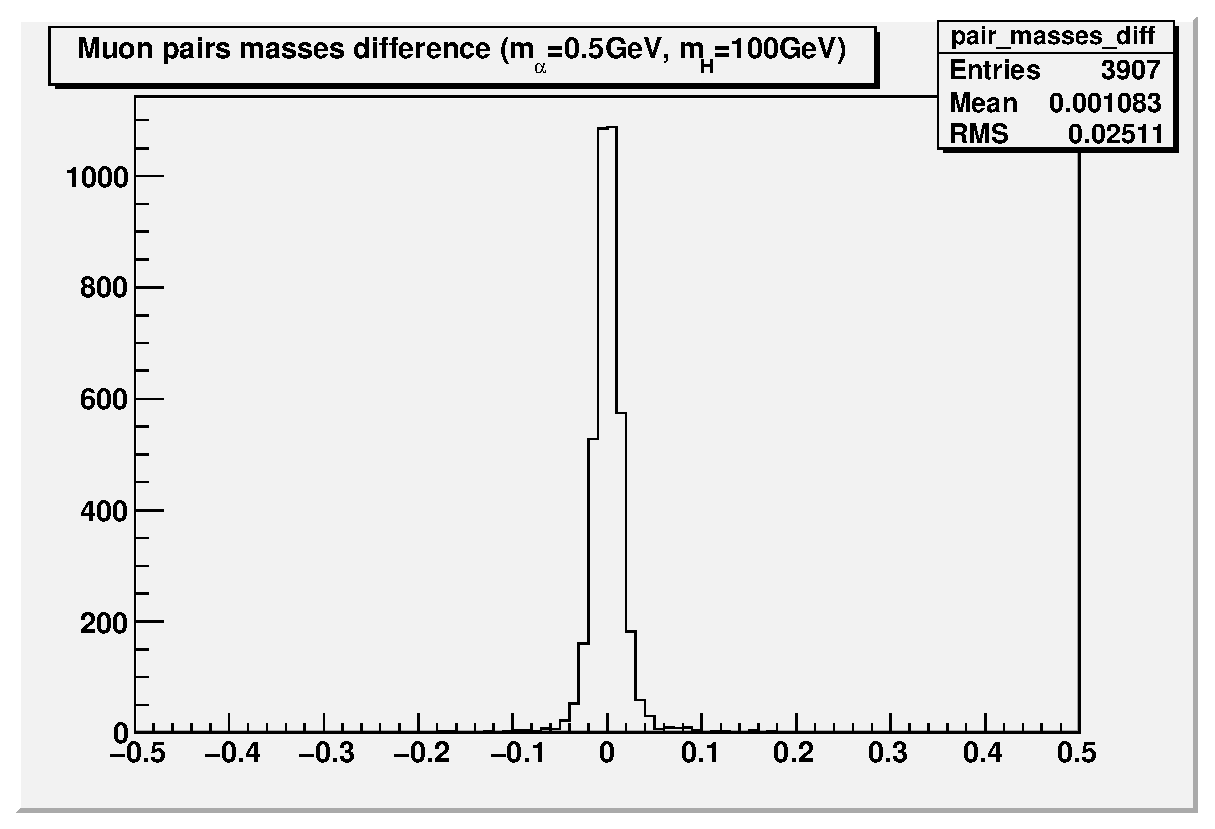
\includegraphics[width=0.48\linewidth]{plots/pairs_masses_diff_0.5.eps}
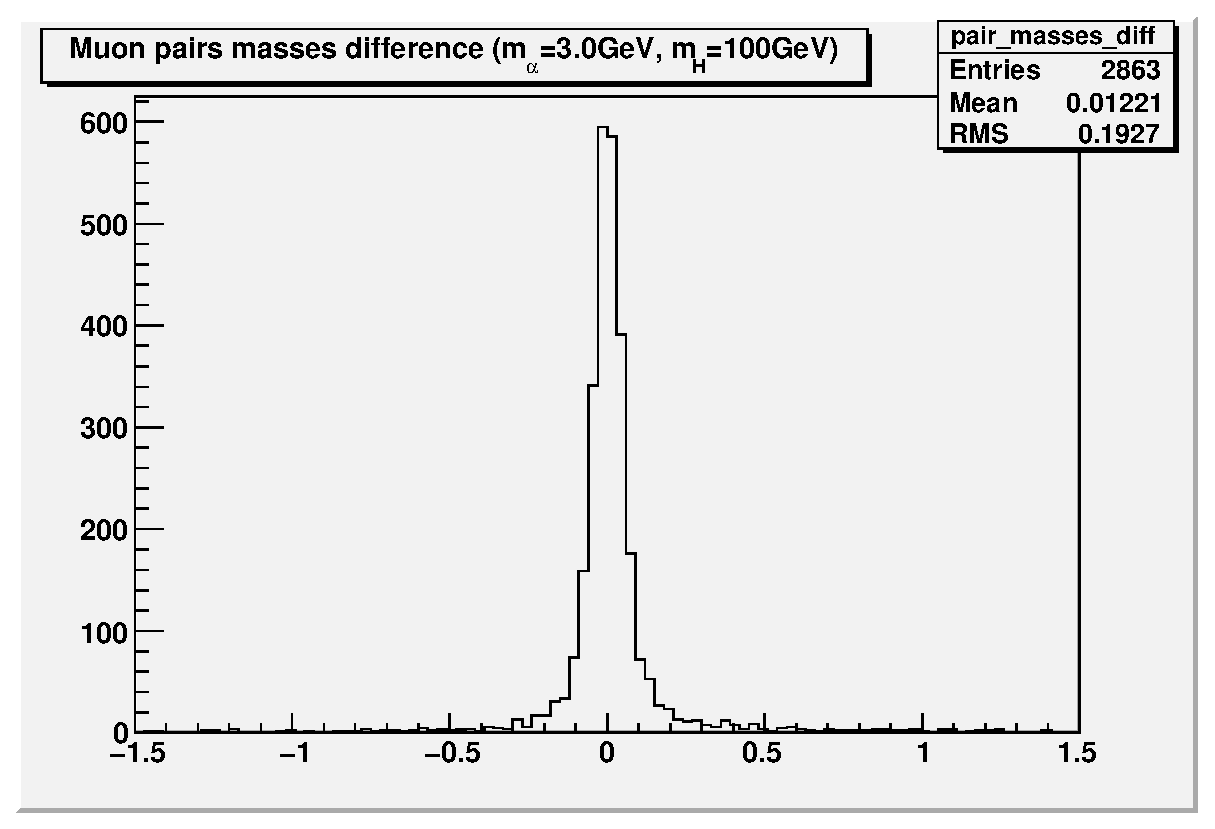
\includegraphics[width=0.48\linewidth]{plots/pairs_masses_diff_3.0.eps}
\caption{Left: Muon pairs masses difference ($m_a$=0.5GeV, $m_H$=100 GeV). 
Right: Muon pairs masses difference ($m_a$=3.0GeV, $m_H$=100 GeV)}
\label{muon_pairs_masses_diff}
\end{center}
\end{figure}

\subsection{Background Estimation}
The main backgrounds in this analysis are QCD multijet events where muons originate
from either heavy flavor quark decays or from $K/\pi$ decays in flight. We also
considered electroweak backgrounds and direct J/psi production, but found those
contributions completely negligible. Requirement of four  sufficiently energetic muons
in the event drastically reduces contributions of all background processes.  Further
constarints on the correlation of di-muon pair masses and relatively high invariant
mass of the four muon system allows an essentially zero background analysis. In the
following we discuss estimation  of these backgrounds.

\subsubsection{QCD backgrounds}

The largest contribution comes from rare QCD multi-jet events with four energetic
reconstructed  muons that are produced either in heavy flavor decays of b and c mesons
(real muons) or in $K/\pi$  decays in flight. The punch-through contamination is
heavily suppresed due to massive shileding  of the CMS muon system.  The multi-jet
background is drastically reduced by the requirement of  at least one muon with
$p_T>20$ GeV/c and the follow up selections. Background events surviving  selections
can be divided into two fractions: events with all four real muons from heavy flavor 
meson decays and events with typically three real muons and a misidentified muon from
$K/\pi$  decays in flight. The first source is estimated using Pythia MC $2 \to 2$ QCD
jet production  by selecting generated muons and smearing distributions using detector
resolutions and efficiencies.  The second contamination is estimated using the same
Pythia sample by selecting events with two  or three real muons and one or more
charged pions or kaons satisfying $p_T$ and $\eta$ requirements  used for muons. Each
such event is assigned a weight calculated as the probability that available $K/\pi$
mesons decay into muons before reaching radius of $\simeq$2 meters ({\bf halfway into
the hadronic  calorimeter - is it what we want?}). We find that the level of
backgrounds due to misidentifications is  comparable to the rate of the backgrounds
associated with real muons from heavy flavor decays.  While the fraction of remaining
events after acceptance cuts does not appear negligible, these events are spread over
the 3D space with only a tiny fraction of them appearing in the region where signal
would appear, see Tables \ref{bckgr_cuts_efficiency_reco_level} and
\ref{bckgr_cuts_number_reco_level}.  If necessary, these remaining backgrounds can be
completely eliminated by applying a loose track isolation  requirement on one of both
of the di-muon pairs.

\subsubsection{Electroweak four lepton backgrounds}

{\bf We use CompHEP to generate a large sample of events with four muons in final
state coming from the electroweak processes. The cross-section of this process is 0.5
pb ({\bf Sasha, is this correct? Kind of sounds very  small!!!}) and after a cut on
the first muon $p_T>20$ GeV/c, the large chunk of remaining events are  $Z\gamma^*$
type events. Very few of these events have muons that can be arranged into pairs with
low invariant  mass, and the fraction of events with similar masses of the pairs is
completely negligible.}

\subsubsection{Other SM Backgrounds}

We also studied several other processes, e.g. direct $J/\psi$ production process that
can produce  a pair of muons with mass in the range of interest of this analysis and
another pair of muons can  come from decays in flight. We used Pythia MC and a
weighing technique similar to the QCD case and  find that this background is
completely negligible. Other SM backgrounds (top, W+jets) are negligible  in the
region of interest of this analysis.

\subsubsection{Summary}

While the number of background events past the acceptance stage and that are used in
the fit is not small,  the fitting procedure described in the next section is
effectively reducing the region of interest to  events that have kinematic properties
of signal events making backgrounds nearly completely negligible, as  illustarted by
the lower part of Table \ref{bckgr_cuts_number_reco_level} showing the number of
expected  background events after each cut in a dataset corresponding to 100 \ipb of
LHC data. {\bf We need a plot  to show background distributions, e.g. m12 and m1234 -
we have them, just need to clean up}.

\begin{table}[t]
\caption{Background cuts efficiency for generator level\label{bckgr_cuts_efficiency_gen_level}}
\begin{center}
\begin{tabular}{|c|c|c|c|}
\hline
%\multicolumn{3}{|c|}{hey}\\ \hline
Cuts & 4 leptons & $\mu+x$ & $J/\Psi$ \\ \hline
1st eta$<$2.4&                 $0.7994\pm0.0040$    &    $0.95638\pm0.00073$       &    $0.0088\pm0.0022$   \\ 
2nd eta$<$2.4&                 $0.8295\pm0.0042$    &    $0.99992\pm0.00003$       &    $1.00^{+0.00}_{-0.06}$ \\ 
3rd eta$<$2.4&                 $0.8541\pm0.0044$    &    $0.99584\pm0.00024$       &    $0.75\pm0.11$       \\ 
4th eta$<$2.4&                 $0.7066\pm0.0061$    &    $0.96407\pm0.00068$       &    $0.75\pm0.13$       \\ 
1st pt$>$5&                    $0.9805\pm0.0022$    &    $1.00000^{+0}_{-0.00001}$ &    $1.0^{+0.0}_{-0.1}$   \\ 
2nd pt$>$5&                    $0.9405\pm0.0038$    &    $0.8676\pm0.0013$         &    $1.0^{+0.0}_{-0.1}$   \\ 
3rd pt$>$5&                    $0.7893\pm0.0068$    &    $0.0445\pm0.0008$         &    $0.3333\pm0.1571$   \\ 
4th pt$>$5&                    $0.4390\pm0.0093$    &    $0.0284\pm0.0032$         &    $0.00^{+0.27}_{-0.00}$  \\ 
1st pt$>$20&                   $0.9524\pm0.0060$    &    $0.9873\pm0.0126$         &    $0$    \\ \hline
analysis acceptance &          $0.1218\pm0.0033$    &    $0.00099\pm0.00011$       &    $0$    \\ \hline
pair masses$<$4&               $0.0025\pm0.0014$    &    $0.3333\pm0.0533$         &    $0$    \\ 
inv. mass$>$60 &               $0.6667\pm0.3333$    &    $0.4231\pm0.0969$         &    $0$    \\ 
$|m_{12}-m_{34}|< 0.08$    &&&\\             
$+0.005*(m_{12}+m_{34})$  &     $X.XXXX\pm X.XXXX$    &    $X.XXXX\pm X.XXXX$         &    $0$    \\ \hline
full efficiency&            $0.000203\pm0.000143$&    $0.00014\pm0.00004$       &    $0$    \\ \hline
\end{tabular}
\end{center}
\end{table}

\begin{table}[t]
\caption{Background cuts efficiency for reco level\label{bckgr_cuts_efficiency_reco_level}}
\begin{center}
\begin{tabular}{|c|c|c|c|}
\hline
%\multicolumn{3}{|c|}{hey}\\ \hline
Cuts & 4 leptons & $\mu+x$  & $J/\Psi$ \\ 
\hline
1st pt$>$5&                    $0.7455\pm0.0044$    &    $1.00000^{+0}_{-0.00001}$   &    $1.0000^{+0}_{-0.0006}$ \\ 
2nd pt$>$5&                    $0.7012\pm0.0053$    &    $1.00000^{+0}_{-0.00001}$   &    $1.0000^{+0}_{-0.0006}$ \\ 
3rd pt$>$5&                    $0.6066\pm0.0068$    &    $0.04349\pm0.0007$          &    $0.3333\pm0.0013$       \\ 
4th pt$>$5&                    $0.3300\pm0.0084$    &    $0.0402\pm0.0034$           &    $0.00^{+0.15}_{-0.00}$  \\ 
1st pt$>$20&                   $0.9573\pm0.0063$    &    $1.000^{+0}_{-0.007}$       &    $0$    \\ 
\hline
analysis acceptance &          $0.1002\pm0.0030$    &    $0.0017\pm0.0002$         &    $0$    \\ 
\hline
pair masses$<$4&               $0.0041\pm0.0020$    &    $0.3358\pm0.0403$           &    $0$    \\ 
inv. mass$>$60 &               $0.50\pm0.25$        &    $0.4348\pm0.0731$           &    $0$    \\ 
$|m_{12}-m_{34}|< 0.08$ GeV   &&&\\       
$+0.005*(m_{12}+m_{34})$ &      $X.XXXX\pm X.XXXX$    &    $X.XXXX\pm X.XXXX$         &    $0$    \\ 
\hline
full efficiency&               $0.00020\pm0.00014$  &    $0.00025\pm0.00006$         &    $0$    \\ 
\hline
\end{tabular}
\end{center}
\end{table}



\begin{table}[t]
\caption{Expected number of background events after each selection cut on generator level\label{bckgr_cuts_number_gen_level}}
\begin{center}
\begin{tabular}{|c|c|c|c|}
\hline
%\multicolumn{3}{|c|}{hey}\\ \hline
Cuts & 4 leptons & Incl. muon & JPsi \\ 
\hline
Initial number&            $48.21\pm0.49$    &    $152878.11\pm546.06$    &    $120.91\pm2.84$   \\ 
1st eta$<$2.4&             $38.54\pm0.43$    &    $146209.61\pm534.01$    &    $1.0652\pm0.2663$ \\ 
2nd eta$<$2.4&             $31.97\pm0.40$    &    $146197.91\pm533.99$    &    $1.0652\pm0.2663$ \\ 
3rd eta$<$2.4&             $27.30\pm0.37$    &    $145589.38\pm532.88$    &    $0.7989\pm0.2306$ \\ 
4th eta$<$2.4&             $19.29\pm0.31$    &    $140358.34\pm523.22$    &    $0.5992\pm0.1997$ \\ 
1st pt$>$5&                $18.92\pm0.30$    &    $140358.34\pm523.22$    &    $0.5992\pm0.1997$ \\ 
2nd pt$>$5&                $17.79\pm0.30$    &    $121774.70\pm487.35$    &    $0.5992\pm0.1997$ \\ 
3rd pt$>$5&                $14.04\pm0.26$    &    $5424.13\pm102.86$      &    $0.1997\pm0.1153$ \\ 
4th pt$>$5&                $6.17\pm0.17$     &    $154.08\pm17.34$        &    $0^{+0.067}_{-0.000}$      \\ 
1st pt$>$20&               $5.87\pm0.17$     &    $152.13\pm17.23$        &    $--$      \\ 
\hline
pair masses$<$4&           $0.0147\pm0.0085$ &    $50.71\pm9.95$          &    $--$      \\ 
inv. mass$>$60 &           $0.0098\pm0.0069$ &    $21.45\pm6.47$          &    $--$      \\ 
$|m_{12}-m_{34}|< 0.08$ GeV  &&&\\       
$+0.005*(m_{12}+m_{34})$ &  $0.000^{+0.005}_{-0.000}$ & {\bf $0.00^{+1.95}_{-0.00}$ ??}  &    $--$    \\ 
\hline
\end{tabular}
\end{center}
\end{table}

\begin{table}[t]
\caption{Expected number of background events after each selection cut on reco level\label{bckgr_cuts_number_reco_level}}
\begin{center}
\begin{tabular}{|c|c|c|c|}
\hline
%\multicolumn{3}{|c|}{hey}\\ \hline
Cuts & 4 leptons & Incl. muon & JPsi \\ 
\hline
Initial number&            $48.21\pm0.49$    &    $152878.11\pm546.06$    &    $120.91\pm2.84$   \\ 
1st pt$>$5&                $35.94\pm0.42$    &    $152878.11\pm546.06$    &    $120.91\pm2.84$   \\ 
2nd pt$>$5&                $21.20\pm0.35$    &    $152878.11\pm546.06$    &    $0.3995\pm0.1631$ \\ 
3rd pt$>$5&                $15.29\pm0.27$    &    $6648.99\pm113.88$      &    $0^{+0.067}_{-0.000}$  \\ 
4th pt$>$5&                $5.04\pm0.16$     &    $267.21\pm22.83$        &    $--$      \\ 
1st pt$>$20&               $4.83\pm0.15$     &    $267.21\pm22.83$        &    $--$      \\ 
\hline
pair masses$<$4&           $0.0049\pm0.0098$ &    $89.72\pm13.23$         &    $--$      \\ 
inv. mass$>$60 &           $0.0098\pm0.0069$ &    $39.01\pm8.72$          &    $--$      \\ 
$|m_{12}-m_{34}|< 0.08$ GeV  &&&\\       
$+0.005*(m_{12}+m_{34})$ &  $0.000^{+0.005}_{-0.000}$ & {\bf $0.00^{+1.95}_{-0.00}$ ??}  &    $--$    \\ 
\hline
\end{tabular}
\end{center}
\end{table}




\section{Statistical Analysis of the Data}

To maximize sensitivity and emulate real data analysis techniques, we define a likelihood function in the 3D space 
$(m_{pair \; 1}, \; m_{pair \; 2}, M)$, where M is the four muon invariant mass. The likelihood is defined as follows:
\begin{eqnarray}
{\cal L}(m_h, m_a, \sigma(pp \to h)) = \prod_i {\cal P}(\sigma(pp \to h) \; L \; BR_{h \to aa} BR^2_{a \to \mu \mu} L
\alpha(m_h, m_a) N^S_i (m_a, m_h) + L \; N^B_i, N^D_i)
\end{eqnarray}
where $i$ runs over bins in 3D space of $(m_{12}, m_{34}, m_{1234})$, $m_h$ is the light higgs mass, $m_a$ is 
axial higgs mass, ${\cal P}(\nu, N)$ is Poisson probability for observing $N$ events when the true rate is $\nu$.
Other parameters are dataset luminosity $L$, acceptance of the signal events $\alpha (m_h, m_a)$ , $N^S_i$ is the 
fraction of reconstructed signal events in bin $i$ ($\Sigma N^S_i = 1$), $N^B_i$ is the rate of background events 
in bin $i$ per unit of luminosity.

Because of the limited statistics in the Monte Carlo samples describing QCD backgrounds, we parameterize the
background distriution in the $(m_{12}, m_{34}, M)$ space using the following function:
\begin{eqnarray}
B(m_{12}, m_{34}, m_{1234}) = f(m_{12}) \times f(m_{34}) \times g(m_{1234}) \\
f(m_{12}) = \\
g(m_{1234}) = ,
\end{eqnarray}
This simple function describes backgrounds very well in the region of interest because typical four muon invariant mass values 
are much larger than the narrow range of di-muon pair masses effectively leading to very little correlation of the two. 
An important note is that using this parameterization requires that in the data analysis the order of pairs has to
be randomized (e.g. designating $m_{12}$ to be the mass of the pair that contains highest $p_T$ muon will break factorization),
and so we randomize them in the analysis. Fitted parameters of the function are shown in Table \ref{table_background_fit_parameters}. 
We verified that background events found in MC are well described by this function by running pseudoexperiments using paramaterized 
distribution and verifying that the p-value for the outcome similar to what is observed in MC is high.

Thus defined likelihood function can be used to calculate the 95\% C.L.\ upper limit on the cross-section times branching ratio
of the $h \to \mu \mu \mu \mu$ signal or determine the intergrated luminosity required to make a discovery at a certain level. 
These results can then be translated into the exclusion region in $(m_a, m_h)$ parameter space or NMSSM parameter space.  
To demonstrate performance of this technique, Figures \ref{likelihood_10pb}a) and b) show calculated likelihood functions 
for two pseudoexperiments, in one of which no signal was injected into the pseudodata and in the other a certain amount of 
signal was admixed in addition to background contributions. In both cases, likelihood function shows expected behavior.

We calculate the 95\% C.L.\ upper limit on the product $\sigma(pp \to h) B_{h \to aa} B^2_{a \to \mu \mu} \, \alpha$, 
using Bayesian technique which is 0.0293~pb at $L = 100$~pb$^{-1}$, approximately 3 events.  In vast majority of 
pseudoexperiments, this limit is independent of $m_h$ and $m_a$ because the effective signal region that dominates 
signal significance in the fitter is essentially background free and probability to observe any pseudodata event is 
very small. Since $B_{a \to \mu\mu}$ is nearly a function of $m_a$ only, it can be factored out, and the corresponding 
upper limit on $\sigma(pp \to h) B_{h \to aa} \alpha$ is presented in Table~\ref{table_bramumu_factorized}.  The upper 
limit on $\sigma(pp \to h) B_{h \to aa}$ is shown as a function of $m_h$ and $m_a$ in Table~\ref{table_both_factorized} 
by factoring out $\alpha$ as well.  Keep in mind that $B_{h \to aa}$ is close to 100\% in much of our preferred region 
of NMSSM parameter space.

\begin{table}[htb]
\caption{95\% C.L.\ on $\sigma(pp \to h) B_{h \to aa} \, \alpha$ at $L = 100$~pb$^{-1}$ as a function of $m_a$, from Fig~\ref{brh4mu_plots}. \label{table_bramumu_factorized}}
\begin{center}
\renewcommand{\arraystretch}{1.1}
\begin{tabular}{| c | c | c |}
\hline
\mbox{\hspace{0.25 cm}}$m_a$ (GeV)\mbox{\hspace{0.25 cm}} & \mbox{\hspace{0.25 cm}}$B_{a \to \mu\mu}$ (\%)\mbox{\hspace{0.25 cm}} & \mbox{\hspace{0.25 cm}}$\sigma(pp \to h) B_{h \to aa} \, \alpha$ (pb)\mbox{\hspace{0.25 cm}} \\\hline
0.5 & 0 & $\infty$ \\
0.75 & 4.2 & 16.5 \\
1.0 & 10.0 & 2.9 \\
1.5 & 15.7 & 1.2 \\
2.0 & 17.2 & 1.0 \\
2.5 & 17.1 & 1.0 \\
3.0 & 16.1 & 1.1 \\
3.5 & 14.8 & 1.3 \\
3.75 & 1.02 & 282 \\
4.0 & 0.73 & 557 \\
5.0 & 0.49 & 1220 \\\hline
\end{tabular}
\end{center}
\end{table}

\begin{table}[htb]
\caption{95\% C.L.\ on $\sigma(pp \to h) B_{h \to aa}$ (pb) at $L = 100$~pb$^{-1}$, from Fig~\ref{brh4mu_plots} and Table~\ref{acceptance}. \label{table_both_factorized}}
\begin{center}
\renewcommand{\arraystretch}{1.3}
\begin{tabular}{| c | c | c | c | c | c |}
\hline
\mbox{\hspace{0.25 cm}}$m_h$, $m_a$ (GeV)\mbox{\hspace{0.25 cm}} & \mbox{\hspace{0.25 cm}}0.5\mbox{\hspace{0.25 cm}} & \mbox{\hspace{0.25 cm}}1.0\mbox{\hspace{0.25 cm}} & \mbox{\hspace{0.25 cm}}2.0\mbox{\hspace{0.25 cm}} & \mbox{\hspace{0.25 cm}}3.0\mbox{\hspace{0.25 cm}} & \mbox{\hspace{0.25 cm}}4.0\mbox{\hspace{0.25 cm}} \\\hline
80 & $\infty$ & 10.9 & 4.1 & 4.6 & 2400 \\\hline
100 & $\infty$ & 8.9 & 3.4 & 3.8 & 2000 \\\hline
120 & $\infty$ & 7.7 & 2.9 & 3.4 & 1800 \\\hline
\end{tabular}
\end{center}
\end{table}

\begin{figure}[htb]
\begin{center}
\includegraphics[width=0.48\linewidth]{plots/likelihood_NoSignal.eps}
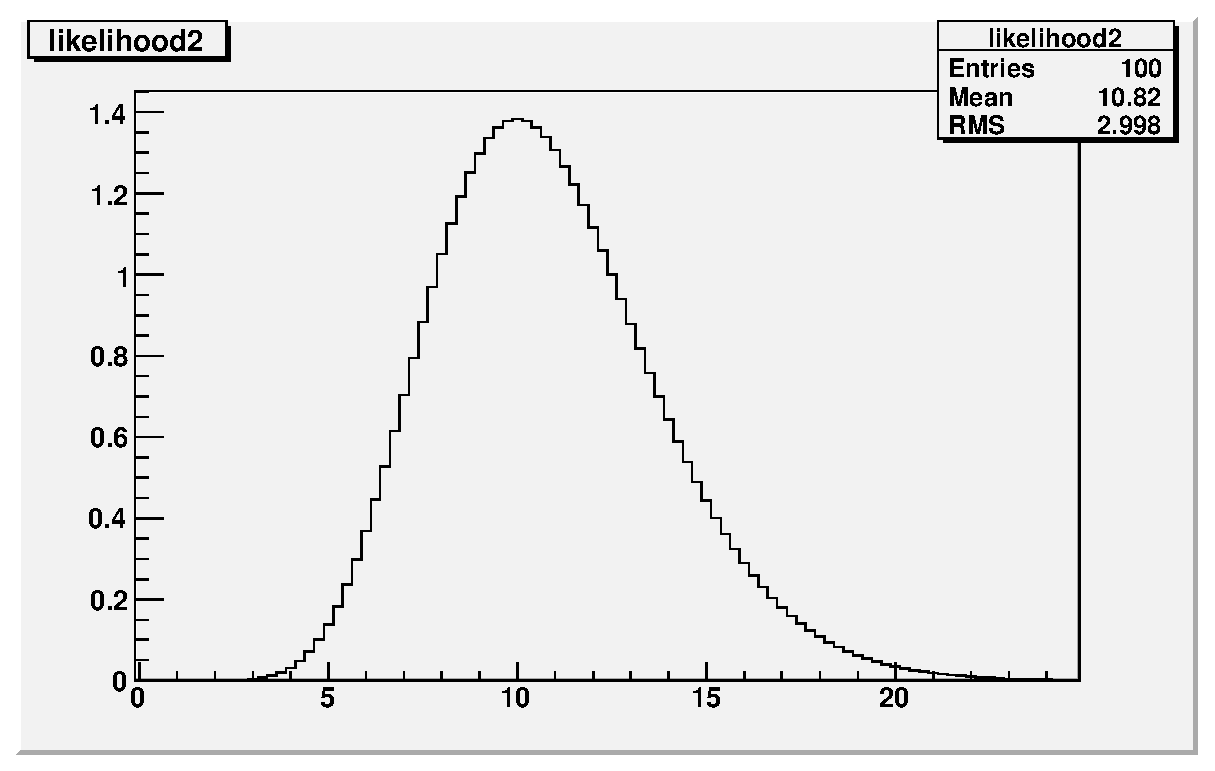
\includegraphics[width=0.48\linewidth]{plots/likelihood_H100_a3_10pb.eps}
\caption{Left:Example likelihood for a pseudoexperiment for a search assuming $B(H \to aa \to \mu \mu \mu \mu)$=0.04, 
$m_a=3$ GeV, $m_h= 100$ GeV with null signal shows that a 95\% exclusion is somewhere around 2.5 pb for  
$\sigma (pp \to H)$. Right: Example likelihood for $\sigma (pp \to H)$=10 \ipb, $B(H \to aa \to \mu \mu \mu \mu)$=0.04, $m_a=3$ GeV 
$m_h= 100$ GeV shows a more than $5 \sigma$ observation.}
\label{likelihood_10pb}
\end{center}
\end{figure}


\section{Results}

{\bf TO BE WRITTEN}

 




%
\section*{Acknowledgments}
We thank XXX and YYY

%\clearpage
%
%  References
%

%%%%%%%%%%%%%%%%%%%%%%%%%%%% References section %%%%%%%%%%%%%%%%%%%%%%%%%%
% A useful Journal macro
\def\Journal#1#2#3#4{{#1} {\bf #2}, #3 (#4)}
% Some useful journal names
\def\NCA{Nuovo Cimento}
\def\NIM{Nucl. Instrum. Methods}
\def\NIMA{{Nucl. Instrum. Methods} A}
\def\NP{Nucl. Phys.} 
\def\NPB{{Nucl. Phys.} B}
\def\PLB{{Phys. Lett.}  B}
\def\PRL{Phys. Rev. Lett.}
\def\RPP{Rep. Prog. Phys.}
\def\PRD{{Phys. Rev.} D}
\def\PR{Phys. Rep.}
\def\PRP{Prog. Theor. Phys.}
\def\ZPC{{Z. Phys.} C}
\def\MPL{{Mod. Phys. Lett.} A}
\def\EPJC{{Eur. Phys. J.} C}
\def\CPC{Comput. Phys. Commun.}

\renewcommand{\baselinestretch}{1}
%\mytableorig

\begin{thebibliography}{99}

\bibitem{Nilles:1982dy}
  H.~P.~Nilles, M.~Srednicki and D.~Wyler,
  %``Weak Interaction Breakdown Induced By Supergravity,''
  Phys.\ Lett.\  B {\bf 120} (1983) 346.
  %%CITATION = PHLTA,B120,346;%%

%\cite{Frere:1983ag}
\bibitem{Frere:1983ag}
  J.~M.~Frere, D.~R.~T.~Jones and S.~Raby,
  %``Fermion Masses And Induction Of The Weak Scale By Supergravity,''
  Nucl.\ Phys.\  B {\bf 222} (1983) 11.
  %%CITATION = NUPHA,B222,11;%%


%\cite{Ellis:1988er}
\bibitem{Ellis:1988er}
  J.~R.~Ellis, J.~F.~Gunion, H.~E.~Haber, L.~Roszkowski and F.~Zwirner,
  %``Higgs Bosons in a Nonminimal Supersymmetric Model,''
  Phys.\ Rev.\  D {\bf 39} (1989) 844.
  %%CITATION = PHRVA,D39,844;%%

%\cite{Drees:1988fc}
\bibitem{Drees:1988fc}
  M.~Drees,
  %``Supersymmetric Models with Extended Higgs Sector,''
  Int.\ J.\ Mod.\ Phys.\  A {\bf 4} (1989) 3635.
  %%CITATION = IMPAE,A4,3635;%%

%\cite{Ellwanger:1993hn}
\bibitem{Ellwanger:1993hn}
  U.~Ellwanger,
  % ``Radiative corrections to the neutral Higgs spectrum in
  %supersymmetry with a gauge singlet,''
  Phys.\ Lett.\  B {\bf 303} (1993) 271
  [arXiv:hep-ph/9302224].
  %%CITATION = PHLTA,B303,271;%%

%\cite{Ellwanger:1993xa}
\bibitem{Ellwanger:1993xa}
  U.~Ellwanger, M.~Rausch de Traubenberg and C.~A.~Savoy,
  %``Particle spectrum in supersymmetric models with a gauge singlet,''
  Phys.\ Lett.\  B {\bf 315} (1993) 331
  [arXiv:hep-ph/9307322].
  %%CITATION = PHLTA,B315,331;%%

%\cite{Elliott:1993bs}
\bibitem{Elliott:1993bs}
  T.~Elliott, S.~F.~King and P.~L.~White,
  % ``Radiative corrections to Higgs boson masses in the next-to-minimal
  %supersymmetric Standard Model,''
  Phys.\ Rev.\  D {\bf 49} 2435 (1994) 2435
  [arXiv:hep-ph/9308309].
  %%CITATION = PHRVA,D49,2435;%%

%\cite{Pandita:1993tg}
\bibitem{Pandita:1993tg}
  P.~N.~Pandita,
  % ``Radiative corrections to the scalar Higgs masses in a nonminimal
  %supersymmetric Standard Model,''
  Z.\ Phys.\  C {\bf 59} (1993) 575.
  %%CITATION = ZEPYA,C59,575;%%

%\cite{Ellwanger:1995ru}
\bibitem{Ellwanger:1995ru}
  U.~Ellwanger, M.~Rausch de Traubenberg and C.~A.~Savoy,
  %``Higgs phenomenology of the supersymmetric model with a gauge singlet,''
  Z.\ Phys.\  C {\bf 67} (1995) 665
  [arXiv:hep-ph/9502206].
  %%CITATION = ZEPYA,C67,665;%%

%\cite{King:1995vk}
\bibitem{King:1995vk}
  S.~F.~King and P.~L.~White,
  % ``Resolving the constrained minimal and next-to-minimal supersymmetric
  %standard models,''
  Phys.\ Rev.\  D {\bf 52} (1995) 4183
  [arXiv:hep-ph/9505326].
  %%CITATION = PHRVA,D52,4183;%%

%\cite{Franke:1995tc}
\bibitem{Franke:1995tc}
  F.~Franke and H.~Fraas,
  % ``Neutralinos and Higgs Bosons in the Next-To-Minimal
  % Supersymmetric Standard Model,''
  Int.\ J.\ Mod.\ Phys.\  A {\bf 12} (1997) 479
  [arXiv:hep-ph/9512366].
  %%CITATION = IMPAE,A12,479;%%

%\cite{Ellwanger:1996gw}
\bibitem{Ellwanger:1996gw}
  U.~Ellwanger, M.~Rausch de Traubenberg and C.~A.~Savoy,
  %``Phenomenology of supersymmetric models with a singlet,''
  Nucl.\ Phys.\  B {\bf 492} (1997) 21
  [arXiv:hep-ph/9611251].
  %%CITATION = NUPHA,B492,21;%%


\bibitem{Miller:2003ay}
  D.~J.~Miller, R.~Nevzorov and P.~M.~Zerwas,
  %``The Higgs sector of the next-to-minimal supersymmetric standard model,''
  Nucl.\ Phys.\  B {\bf 681} (2004) 3.
%  [arXiv:hep-ph/0304049].
  %%CITATION = NUPHA,B681,3;%%
  
\bibitem{mu-problem}
J.~E.~Kim and H.~P.~Nilles,
  %``The Mu Problem And The Strong CP Problem,''
  Phys.\ Lett.\  B {\bf 138}, 150 (1984).

\bibitem{Dermisek:2005ar}
  R.~Dermisek and J.~F.~Gunion,
  %``Escaping the large fine tuning and little hierarchy problems in the  next
  %to minimal supersymmetric model and h --> a a decays,''
  Phys.\ Rev.\ Lett.\  {\bf 95}, 041801 (2005)
  [arXiv:hep-ph/0502105].

\bibitem{nmssm-ph1}
B.~A.~Dobrescu, G.~L.~Landsberg and K.~T.~Matchev,
  %``Higgs boson decays to CP-odd scalars at the Tevatron and beyond,''
  Phys.\ Rev.\  D {\bf 63}, 075003 (2001)
  [arXiv:hep-ph/0005308];
%
 B.~A.~Dobrescu and K.~T.~Matchev,
  %``Light axion within the next-to-minimal supersymmetric standard model,''
  JHEP {\bf 0009}, 031 (2000)
  [arXiv:hep-ph/0008192].
  
\bibitem{nmssm-ph2}
 J.~F.~Gunion, H.~E.~Haber and T.~Moroi,
  %``Will at least one of the Higgs bosons of the next-to-minimal
  %supersymmetric extension of the standard model be observable at LEP2  or the
  %LHC?,''
{\it In the Proceedings of 1996 DPF / DPB Summer Study on New Directions for High-Energy Physics (Snowmass 96), Snowmass, Colorado, 25 Jun - 12
Jul 1996, pp LTH095}
  [arXiv:hep-ph/9610337];
  %
  U.~Ellwanger, J.~F.~Gunion and C.~Hugonie,
  %``Establishing a no-lose theorem for NMSSM Higgs boson discovery at the
  %LHC,''
  arXiv:hep-ph/0111179
  
\bibitem{nmssm-ph2b}
   %
 J.~R.~Ellis, J.~F.~Gunion, H.~E.~Haber, L.~Roszkowski and F.~Zwirner,
  %``Higgs Bosons in a Nonminimal Supersymmetric Model,''
  Phys.\ Rev.\  D {\bf 39}, 844 (1989);
  %
  B.~A.~Dobrescu, G.~L.~Landsberg and K.~T.~Matchev,
  %``Higgs boson decays to CP-odd scalars at the Tevatron and beyond,''
  Phys.\ Rev.\  D {\bf 63}, 075003 (2001)
  [arXiv:hep-ph/0005308];
  
    U.~Ellwanger, J.~F.~Gunion, C.~Hugonie and S.~Moretti,
  %``Towards a no-lose theorem for NMSSM Higgs discovery at the LHC,''
  arXiv:hep-ph/0305109;
  %
   %
  U.~Ellwanger, J.~F.~Gunion, C.~Hugonie and S.~Moretti,
  %``NMSSM Higgs discovery at the LHC,''
  %
  arXiv:hep-ph/0401228;
    U.~Ellwanger, J.~F.~Gunion and C.~Hugonie,
  %``Difficult scenarios for NMSSM Higgs discovery at the LHC,''
  JHEP {\bf 0507}, 041 (2005)
  [arXiv:hep-ph/0503203].
  
 
  
\bibitem{nmssm-ph3}
  S.~Moretti, S.~Munir and P.~Poulose,
  %``Another step towards a no-lose theorem for NMSSM Higgs discovery at the
  %LHC,''
  Phys.\ Lett.\  B {\bf 644}, 241 (2007)
  [arXiv:hep-ph/0608233];
  
  
  
\bibitem{nmssm-ph4}
 S.~Chang, P.~J.~Fox and N.~Weiner,
  %``Visible cascade Higgs decays to four photons at hadron colliders,''
  Phys.\ Rev.\ Lett.\  {\bf 98}, 111802 (2007)
  [arXiv:hep-ph/0608310]. 
  
\bibitem{nmssm-ph5}
  R.~Dermisek and J.~F.~Gunion,
  %``The NMSSM close to the R-symmetry limit and naturalness in h --> aa  decays
  %for m(a) < 2m(b),''
  Phys.\ Rev.\  D {\bf 75}, 075019 (2007)
  [arXiv:hep-ph/0611142].  
  
\bibitem{nmssm-ph6}
 K.~Cheung, J.~Song and Q.~S.~Yan,
  %``Role of h --> eta eta in Intermediate-Mass Higgs Boson Searches at the
  %Large Hadron Collider,''
  Phys.\ Rev.\ Lett.\  {\bf 99}, 031801 (2007)
  [arXiv:hep-ph/0703149]. 

\bibitem{nmssm-ph6a}  
  J.~R.~Forshaw, J.~F.~Gunion, L.~Hodgkinson, A.~Papaefstathiou and A.~D.~Pilkington,
  %``Reinstating the 'no-lose' theorem for NMSSM Higgs discovery at the LHC,''
  JHEP {\bf 0804} (2008) 090
  [arXiv:0712.3510 [hep-ph]].  
  
\bibitem{nmssm-ph7}
  A.~Belyaev, S.~Hesselbach, S.~Lehti, S.~Moretti, 
  A.~Nikitenko and C.~H.~Shepherd-Themistocleous,
  %``The Scope of the 4 tau Channel in Higgs-strahlung and Vector Boson Fusion
  %for the NMSSM No-Lose Theorem at the LHC,''
  arXiv:0805.3505 [hep-ph]. 
  
\bibitem{nmssm-dm}
A.~Menon, D.~E.~Morrissey and C.~E.~M.~Wagner,
  %``Electroweak baryogenesis and dark matter in the nMSSM,''
  Phys.\ Rev.\  D {\bf 70} (2004) 035005
  [arXiv:hep-ph/0404184];
  D.~G.~Cerdeno, C.~Hugonie, D.~E.~Lopez-Fogliani, C.~Munoz and A.~M.~Teixeira,
  %``Theoretical predictions for the direct detection of neutralino dark  matter
  %in the NMSSM,''
  JHEP {\bf 0412} (2004) 048
  [arXiv:hep-ph/0408102];
  %
  G.~Belanger, F.~Boudjema, C.~Hugonie, A.~Pukhov and A.~Semenov,
  %``Relic density of dark matter in the NMSSM,''
  JCAP {\bf 0509}, 001 (2005)
  [arXiv:hep-ph/0505142];
  %
  J.~F.~Gunion, D.~Hooper and B.~McElrath,
  %``Light neutralino dark matter in the NMSSM,''
  Phys.\ Rev.\  D {\bf 73}, 015011 (2006)
  [arXiv:hep-ph/0509024];
  %
  F.~Ferrer, L.~M.~Krauss and S.~Profumo,
  %``Indirect detection of light neutralino dark matter in the NMSSM,''
  Phys.\ Rev.\  D {\bf 74}, 115007 (2006)
  [arXiv:hep-ph/0609257];
  %
   D.~G.~Cerdeno, E.~Gabrielli, D.~E.~Lopez-Fogliani, C.~Munoz and A.~M.~Teixeira,
  %``Phenomenological viability of neutralino dark matter in the NMSSM,''
  JCAP {\bf 0706}, 008 (2007)
  [arXiv:hep-ph/0701271];
  %
  C.~Hugonie, G.~Belanger and A.~Pukhov,
  %``Dark Matter in the Constrained NMSSM,''
  JCAP {\bf 0711}, 009 (2007)
  [arXiv:0707.0628 [hep-ph]];
  %
  V.~Barger, P.~Langacker, I.~Lewis, M.~McCaskey, G.~Shaughnessy and B.~Yencho,
  %``Recoil detection of the lightest neutralino in MSSM singlet extensions,''
  Phys.\ Rev.\  D {\bf 75}, 115002 (2007)
  [arXiv:hep-ph/0702036].
  %
  S.~Kraml, A.~R.~Raklev and M.~J.~White,
  %``NMSSM in disguise: discovering singlino dark matter with soft leptons at
  %the LHC,''
  Phys.\ Lett.\  B {\bf 672}, 361 (2009)
  [arXiv:0811.0011 [hep-ph]];
  %
  G.~Belanger, C.~Hugonie and A.~Pukhov,
  %``Precision measurements, dark matter direct detection and LHC Higgs searches
  %in a constrained NMSSM,''
  JCAP {\bf 0901}, 023 (2009)
  [arXiv:0811.3224 [hep-ph]].
  


%
% CDF detector
%

% \bibitem{ua1-z} C.~Albajar~\etal  (UA1 Collaboration),  \Journal{\PLB}{253}{503}{1991};
% J.~Alitti~\etal  (UA2 Collaboration),  \Journal{\PLB}{276}{365}{1992}.

% \bibitem{lep-wz} The LEP Collaborations: ALEPH, DELPHI, L3 and OPAL, the LEP Electroweak Working Group and the SLD Electroweak
% and Heavy Flavor Working Group (2004), hep-ex/0412015.

% \bibitem{cdf-d0-z} T.~Affolder~\etal (CDF Collaboration), \Journal{\PRL}{84}{845}{2000}; 
% F.~Abe~\etal  (CDF Collaboration), \Journal{\PRD}{59}{052002}{1999}; 
% S.~Abachi~\etal  (D$\O$ Collaboration), \Journal{\PRL}{75}{1456}{1995}; 
% B.~Abbot~\etal {} (D$\O$ Collaboration), \Journal{\PRD}{60}{053003}{1999}. 

% \bibitem{w-z-e} D.~Acosta~\etal  (CDF Collaboration), \Journal{\PRL}{94}{091803}{2005};
% A.~Abulencia~\etal (CDF Collaboration), FERMILAB-PUB-05-360 (2005), Submitted to Phys. Rev. D. 

% \bibitem{D0_ztt} V.M.~Abazov~\etal (D$\O$ Collaboration), \Journal{\PRD}{71}{072004}{2005}.

% \bibitem{run2_susy_higgs_workshop} M.~Carena~\etal, hep-ph/0010338; M.~Carena~\etal, \Journal{\EPJC}{26}{601}{2003}; S.~Abel~\etal, hep-ph/0003154.

% \bibitem{belyaev} S. Belyaev, T. Han, and R. Rosenfeld, \Journal{JHEP}{0307}{021}{2003}.

% \bibitem{susy_golden_mode} A.~Dedes~\etal, hep-ph/0207026.

% \bibitem{CDFditauAnalyses} A. Abulencia~\etal (CDF Collaboration), \Journal{\PRL}{96}{011802}{2006}; 
% D.~Acosta~\etal (CDF Collaboration), \Journal{\PRL}{95}{131801}{2005} .

% \bibitem{CDFrunIhiggs} D. Acosta~\etal (CDF Collaboration), \Journal{\PRD}{72}{072004}{2005}. 

% \bibitem{CDFDetector}  D. Acosta {\em et al.} (CDF Collaboration), \Journal{\PRD}{71}{032001}{2005}.

% \bibitem{lt} S. Baroiant~\etal, \Journal{\NIMA}{518}{609}{2004}.

% \bibitem{CDFLuminosity} S. Klimenko, J. Konigsberg, and T.M. Liss, FERMILAB-FN-0741 (2003). 

% \bibitem{pythia} T. Sjostrand~\etal, \Journal{JHEP}{0207}{012}{2002}.

% \bibitem{CTEQ6} J. Pumplin~\etal, \Journal{\CPC}{135}{238}{2001}.

% \bibitem{D-track_reco} D.~Acosta~\etal (CDF Collaboration), \Journal{\PRL}{91}{241904}{2003}.

% \bibitem{jet-energy-paper} A. Bhatti~\etal, \Journal{\NIMA}{566}{375}{2006}.

% \bibitem{jet-clu} F. Abe~\etal (CDF Collaboration), \Journal{\PRD}{45}{1448}{1992}.

% \bibitem{PDG} Particle Data Group, \Journal{\PLB}{592}{1}{2004}.

% \bibitem{nnlo-x-sec} P. Sutton, A. Martin, R. Roberts, and W. Stirling, \Journal{\PRD}{45}{2349}{1992};
% R. Rijken and W. van Neerven, \Journal{\PRD}{51}{44}{1995};
% R. Hamberg, W. van Neerven, and T. Matsuura, \Journal{\NPB}{359}{343}{1991};
% R. Harlander and W. Kilgore, \Journal{\PRL}{88}{201801}{2002};
% W. van Neerven and E. Zijstra, \Journal{\NPB}{382}{11}{1992}.

% \bibitem{cor-factor-zgamma} A. Martin, R. Roberts, W. Stirling, and R. S. Thorne, \Journal{\EPJC}{28}{455}{2003}.

% \bibitem{geant} R.Brun~\etal, GEANT Detector Description and Simulation Tool, CERN Program Library, W5013, 1994.

% 
% Jim's papers to be merged in

\bibitem{nmssmtools1} U.~Ellwanger, J.F.~Gunion and C.~Hugoine,
\Journal{JHEP}{0502}{066}{2005}.

\bibitem{nmssmtools2} U.~Ellwanger, C.~Hugoine, \Journal{\CPC}{175}{290}{2006}.

\bibitem{nmssmtools3} F.~Domingo and U.~Ellwanger, arXiv:0710.3714 [hep-ph].

\bibitem{lep1exclusion} G.~Abbiendi~\etal (OPAL Collaboration),
\Journal{\EPJC}{18}{425-445}{2001}.

\bibitem{lep2exclusion} G.~Abbiendi~\etal (OPAL Collaboration),
\Journal{\EPJC}{27}{483-495}{2003}, arXiv:0209068v1 [hep-ex].

%\cite{Spira:1995rr}
\bibitem{Spira:1995rr}
  M.~Spira, A.~Djouadi, D.~Graudenz and P.~M.~Zerwas,
  %``Higgs boson production at the LHC,''
  Nucl.\ Phys.\  B {\bf 453}, 17 (1995)
  [arXiv:hep-ph/9504378].
  %%CITATION = NUPHA,B453,17;%%%\cite{Spira:1995mt}

 %\cite{Djouadi:1997yw}
\bibitem{Djouadi:1997yw}
  A.~Djouadi, J.~Kalinowski and M.~Spira,
  %``HDECAY: A program for Higgs boson decays in the standard model and its
  %supersymmetric extension,''
  Comput.\ Phys.\ Commun.\  {\bf 108}, 56 (1998)
  [arXiv:hep-ph/9704448].
  %%CITATION = CPHCB,108,56;%% 

%\cite{Balazs:1998sb}
\bibitem{Balazs:1998sb}
  C.~Balazs, H.~J.~He and C.~P.~Yuan,
  %``QCD corrections to scalar production via heavy quark fusion at hadron
  %colliders,''
  Phys.\ Rev.\  D {\bf 60}, 114001 (1999)
  [arXiv:hep-ph/9812263].
  %%CITATION = PHRVA,D60,114001;%%
  
  
 %\cite{Belyaev:2005nu}
\bibitem{Belyaev:2005nu}
  A.~Belyaev, J.~Pumplin, W.~K.~Tung and C.~P.~Yuan,
  %``Uncertainties of the inclusive Higgs production cross section at the
  %Tevatron and the LHC,''
  JHEP {\bf 0601}, 069 (2006)
  [arXiv:hep-ph/0508222].
  %%CITATION = JHEPA,0601,069;%% 
  
%
% Coordinate for CDF detector
%

%\bibitem{CDFdet} CDF Collaboration, F.~Abe~\etal, \Journal{\NIMA}{271}{387}{1988}.
    
%\bibitem{Topref} CDF Collaboration, F.~Abe~\etal, \Journal{\PRD}{50}{2966}{1994}.
\end{thebibliography}

\section{Appendix}


\begin{table}[t]
\caption{Background samples normalization\label{bckgr_normalize}}
\begin{center}
\begin{tabular}{|c|c|c|c|c|c|}
\hline
%\multicolumn{3}{|c|}{hey}\\ \hline
Sample & $\sigma$ & $N^{gen}_{evt}$ & Filter efficiency & $L_{eff}$ & $f = L_{100}/L_{eff}$ \\ \hline
$\mu+x$ &           $0.5091mb$    &    $6238383$      &    $0.000239$  &  $51.2709pb^{-1}$   &  $1.9504$ \\ \hline
4 leptons &        $0.538pb$     &    $10995$        &    $1.0$       &  $20436.803pb^{-1}$ &  $0.0049$ \\ \hline
$J/\psi$ &         $0.127.2nb$   &    $1413803$      &    $0.0074$    &  $1502.00pb^{-1}$   &  $0.0666$ \\ \hline

\end{tabular}
\end{center}
\end{table}

\end{document}

\bibitem{Djouadi:2008uw}
  A.~Djouadi {\it et al.},
  %``Benchmark scenarios for the NMSSM,''
  arXiv:0801.4321 [hep-ph].
  %%CITATION = ARXIV:0801.4321;%%

%\cite{Djouadi:2008yj}
\bibitem{Djouadi:2008yj}
  A.~Djouadi, U.~Ellwanger and A.~M.~Teixeira,
  %``The constrained next-to-minimal supersymmetric standard model,''
  arXiv:0803.0253 [hep-ph].
  %%CITATION = ARXIV:0803.0253;%%

\bibitem{cNMSSM-benchmarks} 
A. Djouadi, U. Ellwanger, R. Godbole,  
C. Hugonie,  S.F. King,  S. Lehti, 
S. Moretti, A. Nikitenko, 
I. Rottl\"ander,  M. Schumacher and 
A. M. Teixeira, in arXiv:0803.1154 [hep-ph].
